\documentclass[11pt]{article}
\usepackage[a4paper,margin=24mm]{geometry}
\usepackage{fontspec}
\setmainfont{Noto Serif}
\usepackage{microtype}
\usepackage{amsmath,amssymb,mathtools}
\usepackage{booktabs,longtable,array}
\usepackage{algorithm}
\usepackage{algpseudocode}
\usepackage{graphicx}
\usepackage{xurl}
\usepackage{hyperref}
\usepackage{bookmark}
\usepackage{enumitem}
\hypersetup{colorlinks=true,linkcolor=blue,citecolor=blue,urlcolor=blue}
\urlstyle{same}
\setlength{\parindent}{0pt}
\setlength{\parskip}{5pt}
\setlength{\emergencystretch}{3em}
\setcounter{secnumdepth}{2}
\newcommand{\tightlist}{\setlength{\itemsep}{0pt}\setlength{\parskip}{0pt}}
\newcommand{\doctype}{Preprint}
\newcommand{\docversion}{v0.02}
\newcommand{\docdate}{13 November 2026}
\newcommand{\versiondoi}{not-assigned}
\newcommand{\conceptdoi}{not-assigned}
\newcommand{\docrepo}{github.com/fsantibanezleal/CAOS\_Geophysics}
\newcommand{\headerblock}{%
\begin{center}
\fbox{\parbox{0.94\textwidth}{\small\raggedright
\textbf{\doctype} \quad$\cdot$\quad \docversion, \docdate \quad$\cdot$\quad Licence CC BY 4.0\\[2pt]
CAOS Research open-problems programme \quad$\cdot$\quad project Inverse Earth Studio\\[2pt]
Version DOI: not assigned \quad$\cdot$\quad concept DOI (always latest): not assigned\\[2pt]
Not peer reviewed. Source code, data and computational records: \href{https://\docrepo}{\texttt{\docrepo}}
}}
\end{center}
\vspace{4pt}}
\title{Geometry-normalized residual learning for first-arrival traveltime tomography: a controlled synthetic comparison}
\author{Felipe Santib\'a\~nez-Leal}
\date{}
\begin{document}
\maketitle
\headerblock
\begin{abstract}
First-arrival traveltime inversion is underdetermined when ray illumination is incomplete, and a convolutional prior can fit synthetic examples without transferring across geology or acquisition. We evaluate a bounded two-channel residual CNN whose inputs are a path-length-normalized backprojection of pick residuals and normalized cell coverage. The model predicts a velocity field on a fixed 16 by 16 grid from 800 training surveys and 160 validation surveys, then is compared with a validation-selected regularized straight-ray inverse on frozen held-out cohorts. The model is initialized to reproduce the reference velocity exactly, constrained to 1400--4000 m/s, trained for 40 epochs, and selected using validation velocity RMSE. On 160 joint family and acquisition shifts, its velocity RMSE is 2.194 times the matched reference and its travel-time RMSE against the observed noisy picks, computed with a separate bilinear operator, is 5.585 times the reference; every case exceeds a 6.091 ms validation-derived residual threshold. A second CUDA training with the same code, seed, and case manifests produces a distinct checkpoint and joint-shift ratios of 2.190 and 5.595, with all 160 cases above its 6.23 ms validation threshold. Both runs fail the predeclared comparison. The ablations use new test-cohort seeds and are exploratory. These synthetic experiments establish neither field accuracy nor geological transfer, and they do not establish algorithmic novelty.
\end{abstract}

\section{Introduction}
\label{sec:introduction}
First-arrival traveltime tomography estimates a subsurface velocity or slowness field from picked source--receiver travel times. It supports near-surface characterization, static correction, refraction imaging, and the construction of starting models for later wave-equation methods. The basic observation is an integral along a propagation path, so the map from a two-dimensional field to a finite list of travel times discards spatial detail. A visually continuous recovered image therefore does not imply that each displayed cell is independently constrained. Acquisition geometry, pick errors, the forward approximation, parameterization, and regularization jointly define what can be recovered. The classical linearized formulations made this dependence explicit; nonlinear ray bending and finite-frequency effects introduce further model dependence [\cite{AkiLee1976,AkiChristofferson1977,Hole1992,Dahlen2004,Rawlinson2010}].

Learning-based inversion offers a different parameter-to-model map. A network can encode spatial structure learned from synthetic examples and return an estimate without running an iterative inverse for each case. That convenience does not remove nonuniqueness. It transfers part of the prior from an explicit regularizer into the training distribution, architecture, loss, and model-selection rule. Published travel-time learning methods exploit particular acquisition geometries, eikonal constraints, iterative velocity-building workflows, neural parameterizations, or probabilistic ensembles [\cite{FanYing2023,Muller2023,LiEKI2025,Zeng2026,WangSpace2026}]. Their results motivate careful evaluation, but their architectures and datasets differ from the small fixed-grid residual model considered here. A claim about one does not imply performance for another.

We test a specific falsifiable proposition: a dimensionally normalized residual backprojection, supplied with a coverage channel and used to predict a bounded update around a reference model, will reduce both model-space error and $Q$-scored misfit to observed picks relative to a regularized ray inverse on held-out family and acquisition shifts. The bilinear quadrature matrix $Q$ is discretized separately from the cell-ray inversion matrix $A$, but it is also the synthetic data-generating operator; the score is independent of $A$'s discretization, not of the generator. The proposed input calculation addresses a known feature-scaling defect in an earlier experimental implementation. It does not change the fact that the training generator uses straight-ray travel times and a small set of authored synthetic families. The network sees observed picks and geometry at inference; truth is available only during supervised training and test scoring.

The central result is negative. For the locked 160-case joint-shift cohort, learned-to-reference ratios are 2.194 for velocity RMSE and 5.585 for $Q$-scored travel-time RMSE against the observed noisy picks. All 160 predicted models exceed a threshold estimated from validation residuals. The model also fails on the individual in-distribution, family-shift, and acquisition-shift cohorts. A later channel ablation on new test-cohort seeds, with the training seed held fixed, finds that neither residual-only input nor coverage-only input recovers the lost performance. These facts narrow the observed failure for this setup. They do not prove that every residual network fails, nor do the post-hoc ablations independently confirm a general causal explanation.

The contributions are limited to: (i) an executable derivation and implementation of a path-normalized residual and coverage input for a bounded CNN; (ii) a frozen matched comparison with a regularized ray inverse and a separately discretized quadrature scorer; (iii) disjoint generator-seed cohorts for interpolation and three specified shifts; (iv) a hash-bound replay and channel ablations on new test-cohort seeds with the training seed fixed; and (v) an explicit negative finding with case-level uncertainty. No new theorem guarantees learning benefit, and no field-data claim is made. Section~\ref{sec:related} locates the experiment among inverse theory and learned tomography. Sections~\ref{sec:problem}--\ref{sec:method} define the model and method; Section~\ref{sec:theory} states the identifiability boundary; Sections~\ref{sec:design}--\ref{sec:ablation} report the experiment; the remaining sections interpret scope and reproducibility.

\section{Related work}
\label{sec:related}
\subsection{Traveltime inverse problems and resolution}
\label{sec:related-inverse}
The ray-theoretic first-arrival problem is commonly written as a path integral of slowness. Aki and Lee formulated three-dimensional velocity estimation from local-event first arrivals, while subsequent nonlinear formulations couple ray tracing, event geometry, and velocity updates [\cite{AkiLee1976,AkiChristofferson1977,Hole1992}]. Numerical travel-time algorithms solve different forward problems: finite-difference eikonal methods approximate first-arrival fields on grids [\cite{Vidale1988,Podvin1991,MoHarris2002}], while ray-cell matrices encode integrals along prescribed paths. These representations are related but not interchangeable. The benchmark here uses a fixed, straight path matrix for inversion and a separate midpoint quadrature over bilinearly interpolated slowness for scoring. It does not use a bent-ray or eikonal solver.

Resolution depends on illumination and on the model class, not only on data residual. Backus--Gilbert averaging kernels formalize which combinations of model parameters are constrained; discrete inverse analyses express the same problem through rank, singular values, and resolution matrices [\cite{BackusGilbert1968,Menke2018,Aster2018}]. Dahlen derives finite-frequency traveltime resolution effects under particular assumptions and distinguishes them from noise and incomplete coverage [\cite{Dahlen2004}]. The present grid has 256 unknown cell velocities and 128 ray observations per acquisition layout. Its ray operator is therefore rank deficient before regularization, with additional low-sensitivity and unsupported cells. A smoothness penalty selects a stable representative; it does not turn the null-space components into measured structure.

Regularization replaces nonunique exact fit with a preference over solutions. Tikhonov formulations penalize a chosen norm, and the L-curve and related criteria study tradeoffs between data fit and solution structure [\cite{Tikhonov1977,Hansen1992}]. Geophysical practice includes smooth and block-preserving alternatives, including modified total variation for first-arrival tomography [\cite{Constable1987,Jiang2016,Jiang2018}]. Bayesian formulations represent prior and observational uncertainty as distributions rather than a single minimizer [\cite{TarantolaValette1982,ScalesSnieder1997,Zhao2022}]. Our reference is intentionally narrower: a quadratic first-difference penalty in a slowness perturbation, with one scalar strength selected from four candidates by validation velocity RMSE. It is a matched baseline for this experiment, not an exhaustive or universally optimal tomography method.

\subsection{Neural methods for travel-time inversion}
\label{sec:related-neural}
Fan and Ying exploit circular acquisition structure and a filtered-backprojection interpretation to design a learned inverse map for two-dimensional eikonal travel-time tomography [\cite{FanYing2023}]. Their architecture and geometry-specific operator motivate treating acquisition as part of the method definition. Deep-Tomography instead iterates learned updates using migrated subsurface-offset panels, with a distinct objective and data representation [\cite{Muller2023}]. Ensemble Kalman inversion combined with neural parameterization targets high-dimensional velocity models and uncertainty through an ensemble [\cite{LiEKI2025}]. EKtomo jointly optimizes travel-time and velocity networks under eikonal constraints and includes synthetic and field examples [\cite{Zeng2026}]. A space-correlation constrained PINN uses another physics-informed formulation [\cite{WangSpace2026}]. None is reproduced in this experiment, and no numerical comparison with their published metrics would be controlled because datasets, acquisition, parameterization, baselines, and objectives differ.

Several 2026 studies sharpen the comparison boundary. Yang et al. use an untrained deep network to parameterize velocity and minimize travel-time misfit, reporting synthetic tests and an application to Central Chile [\cite{YangDNR2026}]. This is an implicit-prior inverse optimization, not a supervised image-to-image map. The linked data record lists test data and inversion outputs [\cite{YangDNRData2026}], but its file set contains no method source code and its license field is blank. We therefore do not treat it as an executable baseline or redistribute its contents. Wang et al. combine a mesh-free eikonal PINN with reciprocity and well-log constraints, and use Monte Carlo dropout to represent prediction uncertainty for models with irregular topography [\cite{WangReciprocity2026}]. Their 2D and 3D synthetic and geological examples make this a direct methodological neighbor, while its continuous physical formulation, extra priors, uncertainty target, and topography differ from the fixed-grid supervised residual map studied here. The authors provide an MIT-licensed notebook implementation and synthetic examples [\cite{WangReciprocityCode2026}], which we have not executed. Kurosawa's MIMIR preprint represents velocity and a TGV-squared auxiliary field with neural networks and compares against an FMM-LSMR baseline on three synthetic crosswell benchmarks [\cite{KurosawaMimir2026}]. Its explicit higher-order regularizer and matched forward solver are relevant to the present paper's regularization and operator-mismatch limitations, but the 128 by 128 continuous-field setup, 5 percent noise, five-seed protocol, and authored benchmark differ from our 16 by 16 fixed-ray experiment. Its authors release the code, benchmarks, and checkpoints under MIT [\cite{KurosawaMimirCode2026}], but those results are not reproduced here. Separately, Zhang et al. formulate adjoint-state first-arrival tomography on unstructured triangular meshes, combining factored-eikonal fast sweeping with an upwind finite-volume adjoint solve [\cite{ZhangAdjoint2026}]. That formulation addresses irregular topography and differs in both forward operator and parameterization from the fixed straight-ray matrix used here. Li, Hung, and Leung develop a multilayer level-set formulation for multiphase interfaces, with an eikonal forward solve, adjoint-state derivatives, and interface-oriented regularization [\cite{LiHungLeung2026}]. This is a second contemporary classical comparator for structured geological boundaries; it differs from the present fixed-grid supervised estimate in both parameterization and objective. We have not implemented or reproduced either method, so this literature comparison makes no relative-accuracy claim. Tang proposes adaptive loss weights from neural-tangent-kernel traces for a travel-time PINN and reports synthetic and field applications [\cite{TangNTK2026}]; the publisher abstract is the source available for this review, so implementation details beyond that abstract are not asserted. These works are relevant current alternatives, but none supplies a like-for-like result for our authored 16 by 16 experiment.

The method tested here is a direct supervised image-to-image estimate from two grid channels. It does not solve an eikonal equation, optimize a velocity model against field observations at inference, use a learned travel-time field, or sample a posterior. Its closest conceptual relatives are learned inverse maps and residual-update networks, but its input channels are determined by a specified straight-ray operator. That distinction matters: a small CNN can exploit repeated patterns in a generator even when the data map has a large null space. General inverse-imaging analyses warn that learned reconstructions depend on training distributions and may violate data consistency outside their training regime [\cite{McCann2017,AdlerOktem2018,Ongie2020,Arridge2019}].

\subsection{Synthetic benchmarks, shift, and uncertainty}
\label{sec:related-benchmarks}
Large synthetic collections such as OpenFWI were developed to make learned full-waveform inversion comparisons more diverse and reproducible [\cite{Deng2022}]. Travel-time studies similarly need to separate random realizations from changes in geology or acquisition. A random seed split alone can leak the same structural family across partitions; conversely, naming a held-out family does not establish broad geological novelty if the family was authored and known in advance. We therefore label the cohorts by the shift they implement, use generator families only as finite stress conditions, and explicitly state that the fault and salt shapes were known to the study authors. They are new seeded realizations from known templates, not independently sampled geological populations.

Automated arrival picking is a distinct upstream task. PickNet and other waveform classifiers infer pick times from traces, whereas this study begins after picks are provided [\cite{WangPickNet2019,ZhuBeroza2019}]. Pick uncertainty and correlated errors affect the inversion, so the synthetic experiment uses independent Gaussian noise with a fixed standard deviation rather than claiming to model real pick behavior. Uncertainty reporting for an inverse model can refer to noise, posterior spread, repeated training, or sampling variation; these quantities answer different questions [\cite{MosegaardTarantola1995,ScalesSnieder1997}]. We report a paired case-bootstrap interval for each fixed cohort. It captures finite-case variation conditional on one trained checkpoint and generator protocol. It is not an uncertainty interval over training seeds, acquisition populations, geological settings, or measurement processes.

\subsection{Position of the present experiment}
\label{sec:related-position}
The literature contains direct learned inverse maps, physics-constrained neural models, iterative learned velocity building, ensemble inference, and conventional regularized solvers. The present experiment is narrower than each broad method family: a two-input-channel CNN maps a 16 by 16 straight-ray residual feature to a bounded velocity grid. Its evaluation is intentionally paired with a validation-selected quadratic ray inverse on the same generated observations, while a separate bilinear quadrature operator scores predicted models. This comparison tests a specific implementation and does not rank entire research families.

The feature uses path length and cell coverage explicitly. Such normalization addresses units and spatial sampling, but neither operation supplies information absent from the observations. A model may learn the generator's spatial morphology, compensate for systematic bias, or fail when new structures violate learned correlations. The split design tests limited family and acquisition changes, but it cannot determine which mechanism dominates the negative result. The residual-only and coverage-only ablations help identify whether one input alone accounts for the outcome. Since they were designed after the primary held-out outcome was inspected, their estimates are exploratory and cannot be used to revise the primary hypothesis or its acceptance decision.

\section{Problem formulation and notation}
\label{sec:problem}
Let the rectangular domain be $\Omega=[0,800]\times[0,800]$ m, with horizontal coordinate $x$ and positive-down depth $z$. The model comprises $N=16\times16=256$ cells of width $\Delta=50$ m. The cell velocity vector is $\mathbf{v}\in[1400,4000]^N$ m/s, and its cellwise slowness is $\mathbf{s}=\mathbf{v}^{-1}$ in s/m. For a fixed acquisition, the straight-ray path-length matrix $A\in\mathbb{R}_{+}^{M\times N}$ has $A_{ij}$ equal to the length of ray $i$ inside cell $j$, in metres. Each observation is a first-arrival time in seconds. The inverse experiment provides $M=128$ picks: 64 rays between opposite vertical boundaries and 64 between opposite horizontal boundaries.

The idealized inversion map is $\mathbf{t}=A\mathbf{s}+\boldsymbol{\epsilon}$. Synthetic observations are generated by a different operator $Q$ that integrates bilinearly interpolated cell-centre slowness along the same geometric segment, then adds zero-mean Gaussian noise with standard deviation $\sigma_t=1$ ms. Thus, $Q$ and $A$ differ in discretization and constitute a controlled operator mismatch. The observation vector is $\mathbf{y}=Q\mathbf{s}^{\star}+\boldsymbol{\epsilon}$, where $\mathbf{s}^{\star}$ is known only for synthetic training and model-space scoring. Inference receives $A$, source and receiver coordinates, and $\mathbf{y}$; it does not receive $\mathbf{s}^{\star}$ or $\mathbf{v}^{\star}$.

For ray $i$, the path length is $\ell_i=\sum_j A_{ij}$, and cell coverage is $c_j=\sum_iA_{ij}$. The reference velocity is $v_{0,j}=2000+0.35z_j$ m/s, where $z_j$ denotes cell-centre depth in metres. The reference slowness is $s_{0,j}=1/v_{0,j}$. Symbols, units, and their operational use are listed in Table~\ref{tab:notation}. A model error is measured in velocity space; a data error is measured in milliseconds after applying the separately discretized scorer $Q$, which also generates the synthetic observations. The two errors are not interchangeable: a model perturbation in the null space of the measured rays may have little effect on $A\mathbf{s}$ while remaining large in model norm.

The acquisition consists of two crosswell-style rectangular boundary layouts, with source and receiver points drawn on opposite edges and straight segments connecting each pair. The nominal count $M=128$ is an observation count for one layout; it does not mean that 128 independent spatial modes are observed. Rows can be correlated, and some cells receive substantially less ray length than others. Each case uses one declared layout rather than concatenating layouts A, B, and C into a synthetic super-survey. This choice makes acquisition shift interpretable as a change in data geometry and keeps the learned input shape fixed. It also limits conclusions to the finite geometry family encoded by the generator.

The model bounds and depth trend are fixed in the source before held-out evaluation. They are conveniences of the synthetic study, not empirically estimated priors for a named field area. No coordinate reference system, topography, anisotropy, attenuation, source statics, or correlated picking error is modeled. The resulting time series isolates a small set of inversion and feature choices; it cannot be treated as a complete acquisition simulator. A field application would need a declared coordinate frame, a survey-specific forward engine, pick provenance and uncertainty, topographic handling, and an inversion mesh justified by sensitivity and scale. The held-out metrics evaluate only the stated rectangle, grid, and noise process.

\begin{table}[htbp]
\centering\small
\caption{Notation identifies the discrete physical quantities and their units used in the forward, feature, inverse, and scoring calculations.}
\label{tab:notation}
\begin{tabular}{p{0.16\textwidth}p{0.58\textwidth}p{0.16\textwidth}}
\toprule Symbol & Meaning & Unit \\
\midrule
$\Omega,\Delta,x,z$ & rectangular domain, cell width, horizontal coordinate, positive-down depth & m \\
$N,M,k$ & cell count, observation count, and case index & dimensionless \\
$\mathbf{v},\mathbf{v}^{\star},\mathbf{v}_0$ & estimated, true, and reference velocity & m/s \\
$\mathbf{s},\mathbf{s}^{\star},\mathbf{s}_0$ & estimated, true, and reference slowness & s/m \\
$A,Q$ & straight-ray inversion matrix and bilinear data-generation/scoring operator & m \\
$A_{ij},\ell_i,c_j$ & cell path length, total ray length, accumulated cell coverage & m \\
$\mathbf{y},\mathbf{t},\boldsymbol{\epsilon},\sigma_t$ & observed time, predicted time, noise, and noise standard deviation & s, except $\sigma_t$ in ms \\
$d_i,\eta_i,h_j$ & reference residual, path-normalized residual, and cell-averaged residual feature & s; s/m; s/m \\
$r_j,g_j$ & normalized residual and normalized coverage input channels & dimensionless \\
$D_{\ell},D_c,G$ & ray-length and coverage diagonals (m), and cell graph Laplacian (dimensionless) & m; m; 1 \\
$\mathbf{q},\widehat{\mathbf{q}}_{\lambda}$ & dimensionless slowness perturbation and its quadratic-reference estimate & dimensionless \\
$K$ & coverage-normalized residual-feature operator & dimensionless \\
$\lambda$ & quadratic spatial penalty strength & dimensionless in scaled objective \\
$\rho_v,\rho_t$ & learned-to-reference error ratios & dimensionless \\
\bottomrule
\end{tabular}
\end{table}

\section{Proposed method}
\label{sec:method}
\subsection{Path-normalized residual backprojection}
\label{sec:feature}
The initial travel-time residual against the reference model is $\mathbf{d}=\mathbf{y}-A\mathbf{s}_0$. A raw transpose backprojection $A^{\mathsf T}\mathbf{d}$ combines residual magnitude with ray length: long paths contribute more simply because more metres are traversed. To remove this direct path-length factor before accumulation, the method divides each residual by its ray length and then averages the resulting slowness perturbation proxy over the metres of path crossing each cell:
\begin{align}
\ell_i &= \sum_{j=1}^{N} A_{ij}, & c_j &= \sum_{i=1}^{M} A_{ij}, \\
\eta_i &= \frac{y_i - (A\mathbf{s}_0)_i}{\ell_i}, &
h_j &= \begin{cases}\displaystyle \frac{\sum_i A_{ij}\eta_i}{c_j},&c_j>0,\\0,&c_j=0.\end{cases}
\label{eq:feature}
\end{align}
Because $y_i-(A\mathbf{s}_0)_i$ has units s and $\ell_i$ has units m, $\eta_i$ has units s/m. The weighted sum $\sum_i A_{ij}\eta_i$ has units s; division by $c_j$ returns s/m. Unsupported cells are assigned zero residual feature, but their zero coverage remains visible in the second channel. This fill value is an input convention, not evidence that an unsupported cell has zero physical perturbation.

The first channel converts the first-order slowness perturbation to a dimensionless velocity-scale feature. For $s=1/v$, differentiation gives $\delta v\simeq-v_0^2\delta s$. The code therefore sets $r_j=-h_jv_{0,j}^{2}/400$ m/s divided by the fixed 400 m/s scale. The second channel is $g_j=c_j/\max_k c_k$, with zero values for cells outside the rays. Both channels are reshaped in depth-major, then horizontal order to a 16 by 16 tensor. The resulting map is deliberately a smoothed linearized feature: it is not an exact inversion, an adjoint-state gradient for the bilinear scorer, or a posterior mean. Figure~\ref{fig:features} shows the feature for the first joint-shift case, alongside its synthetic truth and ray coverage.

The separate cell-length and bilinear operators matter to interpretation. The cell-length matrix uses explicit segment-cell intersections, while the scoring operator samples the ray and bilinearly interpolates slowness at a fixed density of at least eight samples per cell width. The two are independently implemented and have distinct source hashes. The mismatch prevents the learned and reference models from being rewarded solely for fitting the identical discrete operator used to construct their input, but it remains a synthetic numerical check rather than an empirical field observation. Changing either operator changes the experiment and fails the hash checks on the saved computation files.

\subsection{Scaling, conditioning, and interpretation of the feature}
\label{sec:feature-scaling}
The transformation in Equation~\ref{eq:feature} can be interpreted by linearizing the cell-length forward map around the reference slowness. If the true slowness is $\mathbf{s}_0+\delta\mathbf{s}$ and the inversion operator also generated the data, then the noiseless residual would be $A\delta\mathbf{s}$. Dividing one datum by its total path length forms a path-average slowness perturbation. The subsequent cell accumulation is a weighted average over ray segments that cross a cell. This is a local summary of measured residuals, not the solution of normal equations and not an unbiased estimator of $\delta s_j$.

The exact first-order map from a slowness perturbation to observation residual is
\begin{equation}
\delta\mathbf{t}=A\delta\mathbf{s},\qquad
\delta t_i=\sum_{j=1}^{N}A_{ij}\delta s_j.
\label{eq:linear-forward}
\end{equation}
Here $A_{ij}$ is a length, so each product has units of seconds. Equation~\ref{eq:linear-forward} makes the null-space issue operational: any component of $\delta\mathbf{s}$ invisible to every measured row is invisible to this first-order data map. A transpose operation accumulates sensitivity but does not invert this map. The feature replaces the unscaled accumulation $A^{\mathsf T}\delta\mathbf{t}$ by path-normalized residuals followed by a coverage-weighted cell mean. This removes a direct dependence on total path length in each ray's scalar contribution; it does not whiten noise or account for covariance between cells induced by shared rays.

For the generated noise model, independent time errors have common variance $\sigma_t^2$. After division by $\ell_i$, the variance of each normalized datum is
\begin{equation}
\operatorname{Var}(\eta_i\mid A)=\frac{\sigma_t^2}{\ell_i^2}.
\label{eq:normalized-noise}
\end{equation}
Path normalization equalizes units but makes shorter rays noisier in transformed coordinates. The cell feature $h_j$ is a weighted sum of these values, and two cell features are statistically dependent when the same noisy pick contributes to both. The network is not supplied with this full covariance. A statistically whitened feature would require a covariance model and a different, separately evaluated transformation; that alternative is outside this experiment. The current feature must not be described as a noise-optimal preconditioner.

The conversion from slowness perturbation to velocity perturbation follows from differentiating $v=1/s$:
\begin{equation}
\left.\frac{\partial v}{\partial s}\right|_{s_0}=-\frac{1}{s_0^2}=-v_0^2,
\qquad \delta v\approx -v_0^2\delta s.
\label{eq:velocity-linearization}
\end{equation}
The dimensionless residual channel divides this first-order velocity change by 400 m/s. Its sign is intentional: a positive observed-minus-reference residual tends locally to imply lower velocity along illuminated segments. Since the ray average mixes cells, the sign and amplitude of an individual backprojected pixel do not uniquely determine the local model perturbation. Changing the residual convention changes this channel and requires retraining.

Coverage has units of metres before scaling. Dividing by its largest cell value maps nonzero values to $(0,1]$ and makes the channel invariant to multiplying every ray length by one common unit conversion. The complete input tensor is
\begin{equation}
\mathbf{x}_{j}=\begin{bmatrix}-v_{0,j}^{2}h_j/(400\;\mathrm{m/s})\\c_j/\max_k c_k\end{bmatrix},\qquad \mathbf{x}\in\mathbb{R}^{2\times16\times16}.
\label{eq:input-tensor}
\end{equation}
When every ray is empty, the implementation rejects the record before normalization; it does not divide by zero or silently mark every cell as supported. The admitted layouts have positive maximum coverage. The second channel distinguishes no crossing from at least one crossing, but scalar $c_j$ does not encode azimuthal diversity. Repeated parallel rays can produce high coverage while leaving transverse variations poorly constrained. A directional coverage tensor or a local resolution measure could preserve additional information, but either would change the hypothesis and model input.

Feature scaling also interacts with the bounded output. Let $u_j=\operatorname{logit}((v_{0,j}-1400)/2600)$ and $f_j=F_\theta(\mathbf{x})_j$. Then the output derivative with respect to the network logit is
\begin{equation}
\frac{\partial\widehat v_j}{\partial f_j}=2600\,\sigma(u_j+f_j)\left[1-\sigma(u_j+f_j)\right],
\label{eq:bounded-derivative}
\end{equation}
where $\sigma$ is the logistic function. The derivative is largest at the interval midpoint and tends to zero near either physical bound. Bounding prevents velocities outside this authored generator's range, but can reduce optimization sensitivity as predictions approach a limit. The saved numerical outputs do not contain a preregistered test of saturation as a failure mechanism. A future diagnosis would report logits, active bounds, and gradients for every split and compare them with a separately frozen parameterization.

Finally, the feature is deterministic given the bytes of $A$, $\mathbf{y}$, $\mathbf{s}_0$, and the declared cell order, but it is not invariant to mesh changes. Changing cell size changes $A$, coverage, the convolutional receptive field in metres, and the relation between a pixel and a geological length scale. Interpreting the same 3 by 3 kernels across resolutions would therefore require a mesh-transfer experiment. The 16 by 16 discretization is a computational design choice, not a claim that 50 m cells resolve field structure. Here “geometry-normalized” means specified dimensional scaling of two channels on one fixed grid, not resolution invariance or statistical optimality.

\subsection{Bounded residual network}
\label{sec:network}
The network $F_{\theta}$ receives $[r,g]\in\mathbb{R}^{2\times16\times16}$. A 3 by 3 convolution maps two channels to 24 feature maps, followed by GELU and three residual blocks. Each residual block contains two 3 by 3 convolutions with 24 channels and GELU after the skip addition. A final 1 by 1 convolution maps the 24 channels to one logit update. The final layer is initialized with zero weights and zero bias. The output is a bounded perturbation of the reference model in logit coordinates:
\begin{equation}
\widehat{v}_j=1400+2600\,\operatorname{sigmoid}\!\left(\operatorname{logit}\left(\frac{v_{0,j}-1400}{2600}\right)+F_{\theta}(r,g)_j\right).
\label{eq:bounded}
\end{equation}
At initialization, $F_{\theta}=0$ and $\widehat{\mathbf{v}}=\mathbf{v}_0$ up to float32 arithmetic. The sigmoid enforces $1400<\widehat{v}_j<4000$ m/s for finite logits. The bounds come from the fixed synthetic generator and are not learned from the test set. A logit residual preserves a nonzero gradient throughout most of the physical range and expresses the network as a correction to a physically interpretable starting profile.

Figure~\ref{fig:architecture} sketches the implemented data path. The drawing is a structural view of the code, not an additional computational result. Input order and scaling are controlled by the feature function. Training uses truth labels and predicted straight-ray travel times; inference uses only the observed picks and geometry. This distinction is critical for a user-data claim: if truth were needed to evaluate or construct an inference input, the method would not solve the stated user inverse problem. User survey inference is implemented separately as an exploratory path and must not be interpreted as validated field accuracy.

\subsection{Training objective and model selection}
\label{sec:objective}
The model is trained with Adam at learning rate 0.001, batch size 64, and fixed seed 77213 for 40 epochs. Each update combines normalized supervised velocity error and a forward-time term:
\begin{equation}
\mathcal{L}(\theta)=\frac{1}{BN}\sum_{b,j}\left(\frac{\widehat v_{bj}-v^{\star}_{bj}}{400\,\mathrm{m/s}}\right)^2 + 0.1\,\frac{1}{BM}\sum_{b,i}\left(\frac{(A\widehat{\mathbf{s}}_b)_i-y_{bi}}{0.01\,\mathrm{s}}\right)^2,
\qquad \widehat{s}_{bj}=1/\widehat{v}_{bj}.
\label{eq:loss}
\end{equation}
Here $B$ is the mini-batch size. Training samples are grouped by acquisition layout before batches are drawn so that each epoch processes the fixed A and B subsets. The forward loss is computed with the cell-length operator used in training. It provides a data term but does not change the fact that supervised truth error is the principal selected validation criterion.

After each epoch, the checkpoint with minimum validation velocity RMSE is retained; ties keep the earliest epoch. The full-channel model selected epoch 40. No held-out labels are used for training, checkpoint choice, or threshold setting. The reportable comparison metric is a ratio of mean per-case RMSEs, with lower than one favoring the learned estimate. This differs from selecting the network because it appears smoother or because a picture resembles the truth. The forward threshold is the 95th percentile of the learned model's validation bilinear travel-time RMSE, fixed before evaluating test cohorts. It is a screening threshold, not a calibrated probability of geological failure.

\subsection{Reference inverse and algorithm}
\label{sec:reference}
For each acquisition layout, the reference estimates a dimensionless perturbation $\mathbf{q}$ by minimizing a quadratic Tikhonov objective with a graph-Laplacian penalty [\cite{Tikhonov1977}]. This is a product implementation of discrete first-difference regularization, run on the same observations and test cohorts as the CNN. Define $\widetilde A=A/(10\;\mathrm{m})$ and $\widetilde{\mathbf b}=(\mathbf{y}-A\mathbf{s}_0)/(0.01\;\mathrm{s})$; both are dimensionless. The dimensionless vector $\mathbf q$ represents a slowness correction on the scale $10^{-3}\;\mathrm{s/m}$. The optimizer solves the unconstrained quadratic problem below, then clips the resulting slowness to the stated physical interval. This post-solve clipping is not equivalent to optimizing under box constraints.
\begin{equation}
\begin{aligned}
\widehat{\mathbf q}_{\lambda}&=\arg\min_{\mathbf q\in\mathbb R^N}\Bigl\{
\|\widetilde A\mathbf q-\widetilde{\mathbf b}\|_2^2\\
&\qquad+\lambda\mathbf q^{\mathsf T}G\mathbf q+0.01\|\mathbf q\|_2^2\Bigr\},\\
\widehat{\mathbf{s}}&=\operatorname{clip}\left(\mathbf{s}_0+(10^{-3}\;\mathrm{s/m})\widehat{\mathbf q}_{\lambda},\frac{1}{4000}\;\mathrm{s/m},\frac{1}{1400}\;\mathrm{s/m}\right).
\end{aligned}
\label{eq:reference}
\end{equation}
The matrix $G$ is the unweighted four-neighbour cell graph Laplacian. Its quadratic form penalizes squared differences between adjacent dimensionless perturbations. The small diagonal term makes the normal equations strictly positive definite for the finite matrix. The optimizer evaluates $\lambda\in\{1,10,100,1000\}$ and selects the candidate with lowest validation velocity RMSE; ties select the lower numerical value. The selected value was 100. Table~\ref{tab:parameters} lists these settings and the training choices that define the frozen comparison.

Algorithm~\ref{alg:method} summarizes the one-time train and test workflow. It keeps the validation split separate from the final cohorts. The ray inverse is fitted for each survey using a value selected on validation data, while the network predicts directly. Both outputs use the same truth-independent input records. The scorer applies $Q$ to each predicted slowness and compares with the noisy observed picks when computing the Q-scored observed-pick error. The same observations are used in both inversion paths. The frozen result files provide the cohort counts, selected checkpoint, parameter hashes, and per-case values used in the analysis.

\begin{algorithm}[htbp]
\caption{Train and evaluate bounded residual travel-time refinement under frozen splits.}
\label{alg:method}
\begin{algorithmic}[1]
\Require Ray layouts, fixed generator, training and validation seed ranges, locked test seed ranges
  \State Construct cell-length operator $A$ and separately discretized quadrature operator $Q$
\State Generate training and validation models, picks, residual features, coverage, and split hashes
\State Select $\lambda$ for the regularized ray inverse using validation velocity RMSE
\State Initialize $F_{\theta}$ with a zero final layer and train for exactly 40 epochs
\State Retain the checkpoint with minimum validation velocity RMSE
\State Estimate the 95th percentile of validation bilinear time RMSE as a screening threshold
\ForAll{locked test cohorts}
  \State Generate new locked test cases using the frozen generator and test-cohort seed namespace
  \State Predict velocity with $F_{\theta}$ and with the selected regularized ray inverse
  \State Score velocity error, $Q$-based travel-time error, and threshold exceedance
\EndFor
\State Write hashes, per-case metrics, model state, and configuration into the immutable result bundle
\end{algorithmic}
\end{algorithm}

\begin{figure}[htbp]
\centering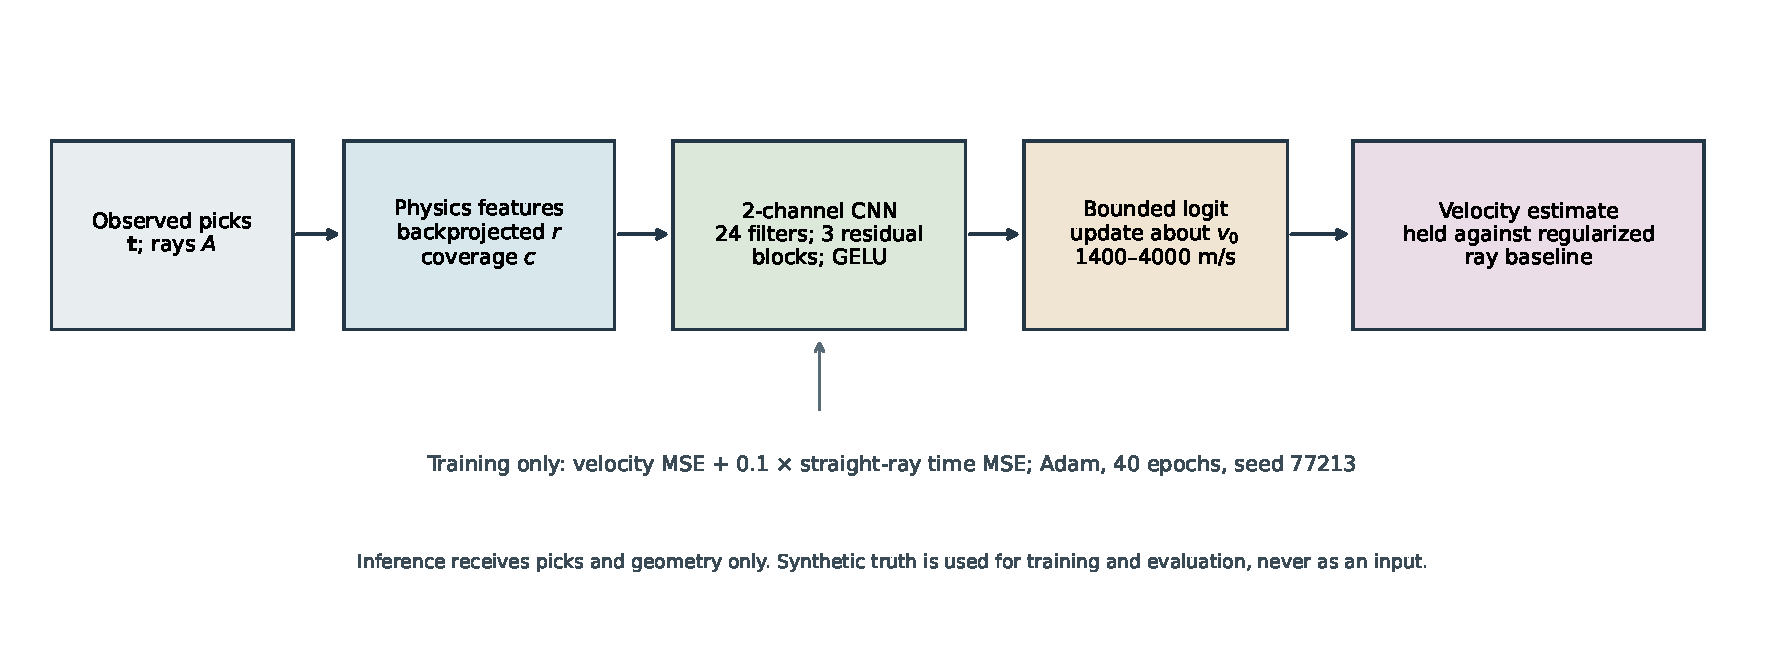
\includegraphics[width=0.98\textwidth]{figures/fig01-method-pipeline.pdf}
\caption{Implemented inference and training paths for the bounded two-channel network, showing where synthetic truth enters and where the reference inverse is compared.}
\label{fig:architecture}
\end{figure}

\section{Theory and identifiability}
\label{sec:theory}
\subsection{A null-space limitation}
\label{sec:nullspace}
For a fixed straight-ray matrix $A$, suppose two slowness fields are related by $\mathbf{s}_2=\mathbf{s}_1+\mathbf{n}$ with $A\mathbf{n}=0$. The linearized travel-time predictions are identical: $A\mathbf{s}_2=A\mathbf{s}_1$. Consequently, no deterministic function of these predicted data alone can distinguish the two fields without additional prior information or another acquisition. This is an algebraic limitation, not a limitation specific to a neural network. It follows directly from the definition of the null space and is consistent with classical resolution analyses [\cite{BackusGilbert1968,Menke2018,Aster2018}].

\begin{equation}
\mathcal{N}(A)=\{\mathbf{n}\in\mathbb{R}^{N}:A\mathbf{n}=\mathbf{0}\},\qquad
\mathbf{n}\in\mathcal{N}(A)\Longrightarrow A(\mathbf{s}+\mathbf{n})=A\mathbf{s}.
\label{eq:nullspace}
\end{equation}
The proof is one line: linearity gives $A(\mathbf{s}+\mathbf{n})=A\mathbf{s}+A\mathbf{n}=A\mathbf{s}$. Since $M=128<N=256$, rank-nullity gives $\dim\mathcal{N}(A)\geq128$ for each layout. Stacking layouts would change the lower bound only if their observations were jointly inverted; the current record uses one selected layout per survey and does not stack A, B, and C into one solve.

The CNN can select one member of an equivalence class by learning correlations in its training family. That selection is a prior encoded in the synthetic distribution. If a held-out model has a different relationship between visible ray integrals and unilluminated cells, the data cannot correct the learned choice. The coverage channel indicates which cells have ray intersections, but a positive coverage value does not establish adequate angular diversity or unique resolution. The residual backprojection adds a local sensitivity-weighted summary but cannot increase the rank of the observations. These distinctions explain why the design is a testable prior rather than a new source of physical information.

\subsection{Resolution-kernel interpretation and measured support}
\label{sec:resolution-kernel}
The feature has an exact linear interpretation under a matched, noiseless ray model. Let $D_{\ell}=\operatorname{diag}(\ell_i)$ and $D_c=\operatorname{diag}(c_j)$, and restrict the cell expression to supported cells where $c_j>0$. If $\mathbf{y}=A(\mathbf{s}_0+\delta\mathbf{s})$, then the unscaled cell feature is
\begin{equation}
\mathbf{h}=D_c^{-1}A^{\mathsf T}D_{\ell}^{-1}A\,\delta\mathbf{s}=K\,\delta\mathbf{s},\qquad
K=D_c^{-1}A^{\mathsf T}D_{\ell}^{-1}A.
\label{eq:feature-resolution}
\end{equation}
The matrix $K$ is a coverage-normalized resolution-like operator. It is generally not the identity, so the feature is a spatially weighted mixture of model perturbations rather than a cellwise recovery. On the supported subspace it is similar to a symmetric positive-semidefinite matrix:
\begin{equation}
D_c^{1/2}KD_c^{-1/2}=D_c^{-1/2}A^{\mathsf T}D_{\ell}^{-1}AD_c^{-1/2}\succeq0.
\label{eq:feature-psd}
\end{equation}
This relation describes the linear smoothing and sensitivity structure, but it does not imply that $K$ is well conditioned. Its rank is bounded by the number of independent rays and can be much lower than the number of supported cells.

In the actual experiment the data use $Q$, not $A$, and include noise. Subtracting the reference prediction gives $\mathbf{y}-A\mathbf{s}_0=A(\mathbf{s}^{\star}-\mathbf{s}_0)+(Q-A)\mathbf{s}^{\star}+\boldsymbol\epsilon$. Thus the feature contains the desired linearized signal passed through $K$, an operator-mismatch term, and noise filtered by the same path and coverage weights. Because $Q$ and $A$ differ, Equation~\ref{eq:feature-resolution} is an explanatory matched-operator limit, not the exact forward equation for the primary experiment. This distinction is necessary to interpret the negative result: the CNN is not given a clean local perturbation map.

For each fixed acquisition layout, we measure the supported-cell count, numerical rank and positive spectrum of the coverage-normalized kernel, as well as the axial ray-angle gaps. Table~\ref{tab:kernel-diagnostics} and Figure~\ref{fig:kernel-spectrum} report these diagnostics from the exact cell-length operators used by the implementation. They expose the finite-dimensional resolution structure of these three discretized layouts: the rank cannot exceed the number of independent ray rows, and a nonzero eigenvalue does not imply useful geological resolution. The spectrum is computed after restricting to cells with positive path coverage and uses a relative eigenvalue cutoff of $10^{-10}$; it is not an empirical estimate of uncertainty or transfer performance.

The diagnostic provides a concrete interpretation of the feature operator, but it does not establish that geometry-conditioned features reduce variance. We did not compare the learned network with a pointwise image prior, nor test a preregistered relation between kernel spectrum and held-out error. The paper therefore makes no such benefit conjecture. Its empirical claim remains the finite synthetic comparison reported below, which is negative under the tested families, noise and acquisition shifts.

\begin{figure}[htbp]
\centering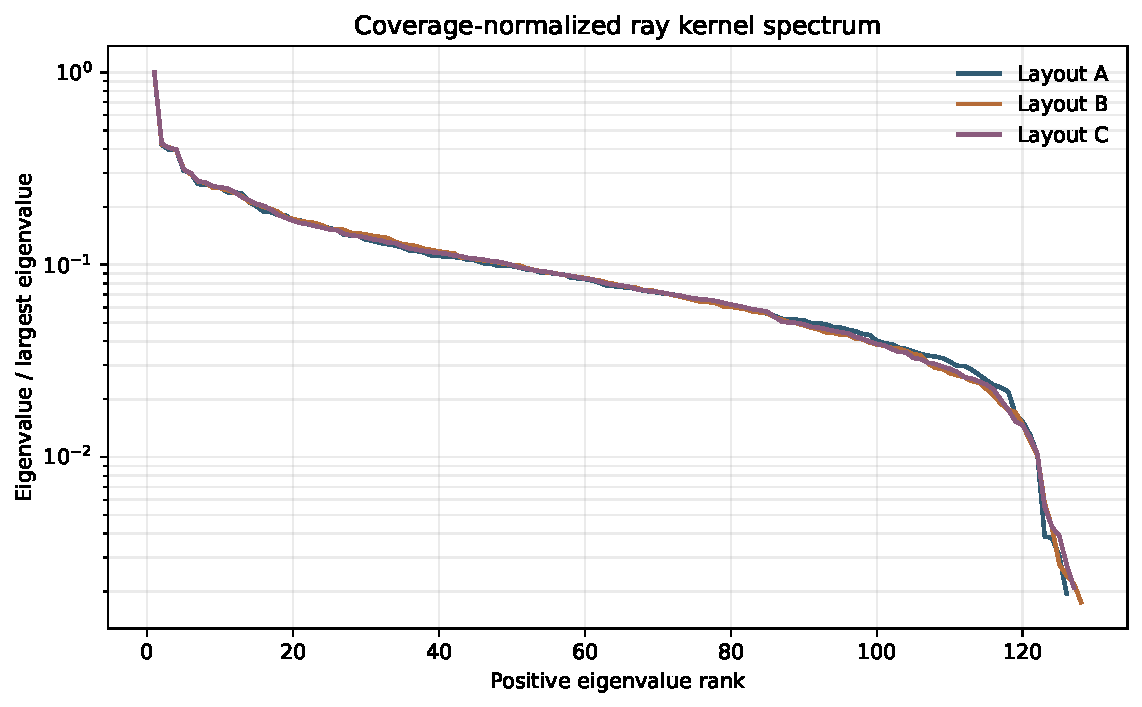
\includegraphics[width=0.78\textwidth]{figures/fig07-resolution-kernel-spectrum.pdf}
\caption{Positive eigenvalues of the coverage-normalized kernel for each fixed acquisition layout show the discrete rank structure, not geological uncertainty or field resolution.}
\label{fig:kernel-spectrum}
\end{figure}

\subsection{What the experiment can and cannot support}
\label{sec:theory-scope}
The null-space proposition does not predict that the learned estimate must be worse than a regularized reference. A prior may reduce expected error under a distribution matched to training, and a learned map may approximate a useful regularization rule. Conversely, the proposition prevents interpreting the network's fine spatial texture as information uniquely recovered from the picks. The relevant empirical question is whether, for the specified family and acquisition distribution, its prior yields lower error than a competitive truth-independent reference. This experiment answers that finite synthetic question negatively under its registered metric.

The outcome is conditional on model dimension, ray geometry, generator, observation noise, objective weights, training seed, checkpoint-selection rule, and baseline candidate set. The observed ratios do not establish universal dominance of quadratic regularization over learned methods. They also do not estimate the benefit of retraining across random seeds. A positive result under another generator or solver would be a separate scientific finding and require a new split, independent reference, complete per-case uncertainty, and appropriate field or external-benchmark evidence. No theoretical convergence or consistency guarantee is asserted for $F_{\theta}$.

\section{Experimental design}
\label{sec:design}
\subsection{Synthetic generator and partitioning}
\label{sec:generator}
The domain, grid, reference profile, noise scale, ray geometry, and all family parameters are implemented in \url{data-pipeline/velocity_validation.py} and \url{data-pipeline/velocity_physics_refinement.py}. Three families appear in both training and validation: smoothly layered interfaces, elliptical velocity lenses, and dipping interfaces. Two additional authored families, faulted interfaces and high-velocity salt bodies, are withheld from training for the family-shift cohort. Acquisition layouts A and B are used for training and validation. Layout C is withheld as an acquisition shift. The joint-shift test combines the known fault/salt families with layout C. Table~\ref{tab:cohorts} gives seed bases and sample counts.

Seed namespaces are disjoint: training starts at 117001, validation at 127001, in-distribution testing at 137001, family shift at 147001, acquisition shift at 157001, and joint shift at 167001. There are 800 training, 160 validation, 160 in-distribution, 80 family-shift, 80 acquisition-shift, and 160 joint-shift cases. Every synthetic model is generated from its seed and family definition, the bilinear operator supplies noiseless times, and independent 1 ms Gaussian perturbations create observed picks. Manifest entries bind each record's family, acquisition, velocity bytes, and noisy-pick bytes by SHA-256. These are repeated realizations from known authored families, not a sample of geological diversity.

\subsection{Comparators and metrics}
\label{sec:metrics}
The primary learned estimate is the frozen 40-epoch checkpoint. The numerical reference is the regularized ray inverse with post-solve physical clipping in Equation~\ref{eq:reference}, with $\lambda$ selected only on validation. Both methods receive the same geometry and noisy picks. The model metric for case $k$ is the root mean squared cell-velocity difference $e_{v,k}=\sqrt{N^{-1}\sum_j(\widehat v_{kj}-v^{\star}_{kj})^2}$ in m/s. For data-space evaluation, predicted slowness is integrated with $Q$ and compared with the same noisy observed picks $\mathbf{y}_k$ used by both methods, giving $e_{t,k}=10^3\sqrt{M^{-1}\|Q\widehat{\mathbf{s}}_k-\mathbf{y}_k\|_2^2}$ in ms. The scorer uses a separate discretization from the inversion matrix, but its residual is not compared with noiseless truth. The model truth is evaluator-only; neither method receives it at inference.

The per-case velocity and travel-time metrics are
\begin{equation}
e_{v,k}=\sqrt{\frac{1}{N}\sum_{j=1}^{N}(\widehat v_{kj}-v^\star_{kj})^2},\qquad
e_{t,k}=10^3\sqrt{\frac{1}{M}\sum_{i=1}^{M}[(Q\widehat{\mathbf{s}}_k)_i-y_{ki}]^2}.
\label{eq:case-metrics}
\end{equation}
The first requires synthetic truth and is unavailable for field observations. The second measures misfit to the observed picks, which include the generated noise, using the bilinear quadrature operator. It is not an error against noiseless travel-time truth. This distinction matters because a method that perfectly reproduces noisy observations can be overfitting the noise, while a lower noisy-pick misfit does not guarantee a lower model error.

For a cohort $C$ with $K$ cases, the reported ratio of mean case errors is
\begin{equation}
\rho_C=\frac{K^{-1}\sum_{k\in C}e_{\mathrm{learned},k}}{K^{-1}\sum_{k\in C}e_{\mathrm{reference},k}}.
\label{eq:ratio}
\end{equation}
Thus $\rho_C>1$ means the learned model has greater average per-case error. The statistic is a ratio of arithmetic means, not a mean of per-case ratios; these summaries differ when the reference errors vary substantially. The paired percentile bootstrap resamples the $K$ case indices with replacement 20,000 times using NumPy PCG64 and fixed seed 6120226 plus a metric/cohort offset. For bootstrap draw $b$, it recomputes the numerator and denominator from the same sampled indices:
\begin{equation}
\rho_C^{(b)}=\frac{\sum_{k\in I_b}e_{\mathrm{learned},k}}{\sum_{k\in I_b}e_{\mathrm{reference},k}},\qquad
\mathrm{CI}_{95\%}=\left[Q_{0.025}(\rho_C^{(b)}),Q_{0.975}(\rho_C^{(b)})\right].
\label{eq:paired-bootstrap}
\end{equation}
The empirical quantiles describe finite-case sampling conditional on one trained checkpoint and this synthetic generator. Pairing preserves the same underlying survey in both methods, but it does not model uncertainty over training seeds, families beyond those authored, or measurement processes absent from the generator. A narrow interval therefore cannot be interpreted as broad geological confidence.

\subsection{Predeclared outcome rule and ablation status}
\label{sec:outcome-rule}
The primary advantage rule requires both velocity and observed-pick travel-time ratios below one on the joint-shift cohort. The threshold-exceedance count is a separate diagnostic: the 95th percentile of validation learned travel-time RMSE is fixed at 6.091015 ms, and every joint-shift model with an error above this value is counted. In symbols, if $\tau$ is the fixed validation quantile, the reported count is
\begin{equation}
n_{\mathrm{flag}}=\sum_{k\in C_{\mathrm{joint}}}\mathbb{1}[e_{t,k}>\tau],\qquad \tau=6.091015\;\mathrm{ms}.
\label{eq:flags}
\end{equation}
These checks answer different questions. The ratios compare aggregate paired errors with the reference; the threshold flags count cases outside a validation-derived error screen. Neither flag frequency nor bootstrap intervals are calibrated failure probabilities for field surveys. The fixed quantile is also estimated from a finite validation set, and its sampling uncertainty is not included in the case bootstrap. Re-estimating the threshold after examining test cases would invalidate the stated protocol, so the reported value remains fixed even when all joint-shift cases exceed it.

The residual-only and coverage-only ablations were designed after the primary test outcome had been inspected. They reuse the frozen training and validation cohort definitions, train from scratch with the same training seed and 40-epoch budget, and are scored on new test-cohort seed bases 177001, 187001, 197001, and 207001. The full-channel model in this follow-up is the original checkpoint, not a retrained third model. The ablation results are therefore exploratory mechanism probes. They cannot be used to tune, replace, or retroactively confirm the primary test. Separate validation thresholds are estimated for each model and are not directly comparable as calibrated quantities.

\begin{table}[htbp]
\centering
\small
\caption{Frozen synthetic cohorts separate interpolation, family shift, acquisition shift, and their joint combination across the declared two-dimensional ray layouts.}
\label{tab:cohorts}
\begin{tabular}{lrrll}
\toprule
Cohort & $n$ & Seed base & Families & Acquisition layouts \\
\midrule
Training & 800 & 117001 & layered, lens, dipping & A, B \\
Validation & 160 & 127001 & layered, lens, dipping & A, B \\
In-distribution test & 160 & 137001 & layered, lens, dipping & A, B \\
Family-shift test & 80 & 147001 & fault, salt & A, B \\
Acquisition-shift test & 80 & 157001 & layered, lens, dipping & C \\
Joint-shift test & 160 & 167001 & fault, salt & C \\
\bottomrule
\end{tabular}
\end{table}

\begin{table}[htbp]
\centering
\small
\caption{The frozen learned model is compared with a validation-selected regularized ray inverse on identical held-out cases.}
\label{tab:primary}
\begin{tabular}{lrrrrr}
\toprule
Cohort & $n$ & Velocity ratio (95\% CI) & Time ratio (95\% CI) & Flags \\
\midrule
In distribution & 160 & 3.034 (2.942, 3.124) & 4.957 (4.748, 5.172) & 14 \\
Family shift & 80 & 2.178 (2.097, 2.275) & 5.733 (5.626, 5.840) & 80 \\
Acquisition shift & 80 & 3.092 (2.961, 3.229) & 5.268 (4.987, 5.576) & 6 \\
Joint shift & 160 & 2.194 (2.133, 2.264) & 5.585 (5.509, 5.662) & 160 \\
\bottomrule
\end{tabular}
\end{table}

\begin{table}[htbp]
\centering
\scriptsize
\caption{Channel-ablation models evaluated on new test-cohort seeds retain larger errors than the matched inverse across every held-out synthetic cohort; the training seed is unchanged.}
\label{tab:ablation}
\begin{tabular}{llrrr}
\toprule
Model & Cohort & Velocity ratio (95\% CI) & Time ratio (95\% CI) & Flags \\
\midrule
Both channels & In distribution & 2.877 (2.792, 2.964) & 4.731 (4.542, 4.920) & 8 \\
Residual only & In distribution & 3.419 (3.319, 3.519) & 4.985 (4.771, 5.207) & 7 \\
Coverage only & In distribution & 11.098 (10.496, 11.705) & 27.711 (26.759, 28.650) & 8 \\
Both channels & Family shift & 2.220 (2.136, 2.322) & 5.616 (5.506, 5.728) & 80 \\
Residual only & Family shift & 2.344 (2.237, 2.473) & 5.860 (5.725, 6.002) & 80 \\
Coverage only & Family shift & 3.642 (3.302, 4.054) & 12.868 (11.947, 13.834) & 22 \\
Both channels & Acquisition shift & 3.080 (2.949, 3.217) & 5.417 (5.128, 5.733) & 8 \\
Residual only & Acquisition shift & 3.467 (3.326, 3.612) & 5.457 (5.109, 5.822) & 8 \\
Coverage only & Acquisition shift & 10.987 (10.080, 11.906) & 28.635 (27.309, 30.010) & 6 \\
Both channels & Joint shift & 2.216 (2.153, 2.289) & 5.597 (5.515, 5.680) & 160 \\
Residual only & Joint shift & 2.327 (2.252, 2.412) & 5.757 (5.665, 5.850) & 160 \\
Coverage only & Joint shift & 3.597 (3.358, 3.877) & 12.765 (12.170, 13.370) & 51 \\
\bottomrule
\end{tabular}
\end{table}

\begin{table}[htbp]
\centering
\small
\caption{Model and solver settings define the trained convolutional estimate and validation-selected ray inverse used for every held-out synthetic cohort.}
\label{tab:parameters}
\begin{tabular}{ll}
\toprule
Quantity & Value \\
\midrule
Grid and domain & $16\times16$, $800\times800$ m, 50 m cells \\
Velocity bounds & 1400--4000 m/s \\
Training cases / validation cases & 800 / 160 \\
Optimizer / learning rate / epochs & Adam / 0.001 / 40 \\
Mini-batch / initialization seed & 64 / 77213 \\
Training objective scales & 400 m/s for velocity; 10 ms for travel time \\
Ray-inverse candidates / selected value & 1, 10, 100, 1000 / 100 \\
Held-out family / acquisition layouts & fault and salt / C \\
Primary selected epoch & 40 \\
Primary GPU training time & 37.51 s \\
Ablation GPU training and scoring time & 30.45 s \\
\bottomrule
\end{tabular}
\end{table}

\clearpage
\begin{table}[htbp]
\centering
\small
\caption{Coverage and eigenvalue summaries quantify rank and angular support of each fixed straight-ray acquisition layout on the 16 by 16 grid.}
\label{tab:kernel-diagnostics}
\begin{tabular}{lrrrrrr}
\toprule
Layout & Rays & Supported cells & Rank & Support (\%) & Axial angles & Max gap ($^\circ$) \\
\midrule
A & 128 & 252 & 126 & 98.4 & 128 & 11.30 \\
B & 128 & 254 & 128 & 99.2 & 128 & 10.96 \\
C & 128 & 251 & 127 & 98.0 & 116 & 11.64 \\
\bottomrule
\end{tabular}
\end{table}


\section{Results}
\label{sec:results}
\subsection{Primary frozen comparison}
\label{sec:primary-results}
The full-channel model selected epoch 40, with validation velocity RMSE 49.763 m/s. The regularized ray baseline selected $\lambda=100$ from candidates 1, 10, 100, and 1000. On the joint-shift set, learned velocity RMSE is 206.837 m/s compared with 94.265 m/s for the baseline. $Q$-scored observed-pick travel-time RMSE is 12.948 ms versus 2.318 ms. The learned-to-reference ratios are 2.194 (case-bootstrap 95\% interval 2.133--2.264) and 5.585 (5.509--5.662), respectively. All 160 of 160 joint-shift cases exceed the 6.091 ms validation threshold. The prespecified criterion requiring both ratios below one is not satisfied.

The other test cohorts show the same direction. Velocity and $Q$-scored travel-time ratios are 3.034 and 4.957 in-distribution, 2.178 and 5.733 under family shift, and 3.092 and 5.268 under acquisition shift. The difference is not confined to the joint shift, although that cohort combines the two held-out conditions and remains the primary test. Figure~\ref{fig:primary-ratios} displays cohort ratios and their paired intervals. Figure~\ref{fig:paired-errors} shows per-case joint-shift errors: points lie above the equality line when the learned estimate has larger error than the reference. Table~\ref{tab:primary} includes the full cohort counts and validation-threshold flags.

The negative comparison is also present on validation data: the selected learned checkpoint's velocity RMSE is 49.763 m/s, while validation selected the ray-reference penalty using the same split. Thus the disparity is not confined to the shifted test families, although validation error cannot replace the locked test result. On the joint cohort, the $Q$-scored travel-time residual is more than five times the reference value. This difference indicates that the learned field is not merely a different model that preserves similar fit to the observed picks. It still does not identify whether training-distribution bias, the operator mismatch, the loss weighting, or another component is the dominant cause.

\subsection{Sensitivity to an independent CUDA training replay}
\label{sec:replay-sensitivity}
An independent CUDA execution used the same training source hash, random seed, epoch budget, synthetic generator, and validation and test case manifests as the primary run. The case-manifest hashes match exactly, and the data and classical reference errors are therefore paired case by case. The checkpoint hashes differ, so the model weights are not bitwise reproducible under this execution environment. This is a training-replay comparison, not a new test cohort or an independent random-seed experiment.

The second checkpoint retains the same negative direction in every held-out cohort. Its learned-to-reference velocity and observed-pick travel-time ratios are 3.050 and 5.128 for the in-distribution cohort, 2.174 and 5.741 for family shift, 3.108 and 5.427 for acquisition shift, and 2.190 and 5.595 for joint shift. All 160 joint-shift cases exceed the replay's validation-derived threshold of 6.232811 ms. The primary checkpoint produced ratios 2.194 and 5.585 on those same cases and a 6.091015 ms threshold. Figure~\ref{fig:replay-sensitivity} and Table~\ref{tab:replay-sensitivity} show that the modest numerical variation does not change the outcome under the predeclared rule.

The case-bootstrap intervals in Figure~\ref{fig:replay-sensitivity} condition on each fixed checkpoint and resample cases. They do not quantify variation across training seeds, devices, or software stacks. Because both CUDA runs used the same seed, their difference measures execution-level sensitivity under one initialization rather than initialization uncertainty. The result supports stability of the negative comparison for these two checkpoints only; it is not a substitute for a multi-seed analysis.

\begin{table}[htbp]
\centering
\small
\caption{A second CUDA training uses the same source, seed, and case manifests but a distinct checkpoint; both runs retain the negative comparison.}
\label{tab:replay-sensitivity}
\begin{tabular}{lrrr}
\toprule
Cohort & Velocity ratio, first / replay & Time ratio, first / replay & Flags, first / replay \\
\midrule
In distribution & 3.034 / 3.050 & 4.957 / 5.128 & 14/12 \\
Family shift & 2.178 / 2.174 & 5.733 / 5.740 & 80/80 \\
Acquisition shift & 3.092 / 3.107 & 5.268 / 5.427 & 6/7 \\
Joint shift & 2.194 / 2.190 & 5.585 / 5.595 & 160/160 \\
\bottomrule
\end{tabular}
\end{table}


\begin{figure}[htbp]
\centering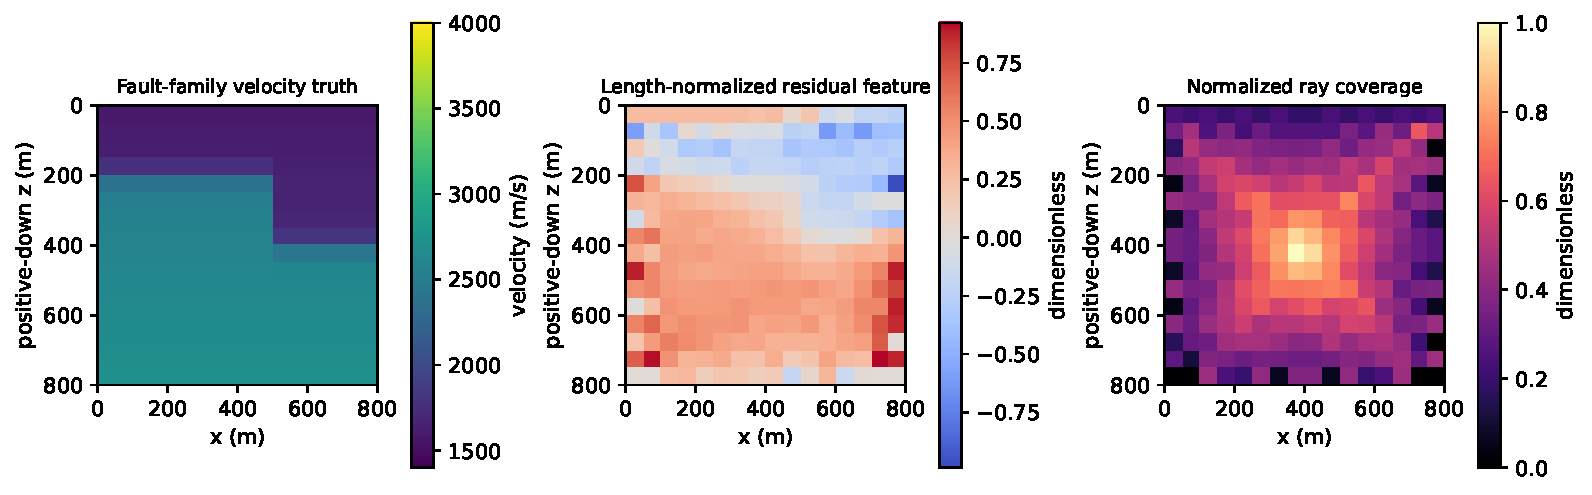
\includegraphics[width=0.98\textwidth]{figures/fig02-input-feature-example.pdf}
\caption{A generated fault-family test example pairs synthetic velocity truth with the length-normalized residual and coverage channels on the fixed acquisition.}
\label{fig:features}
\end{figure}

\begin{figure}[htbp]
\centering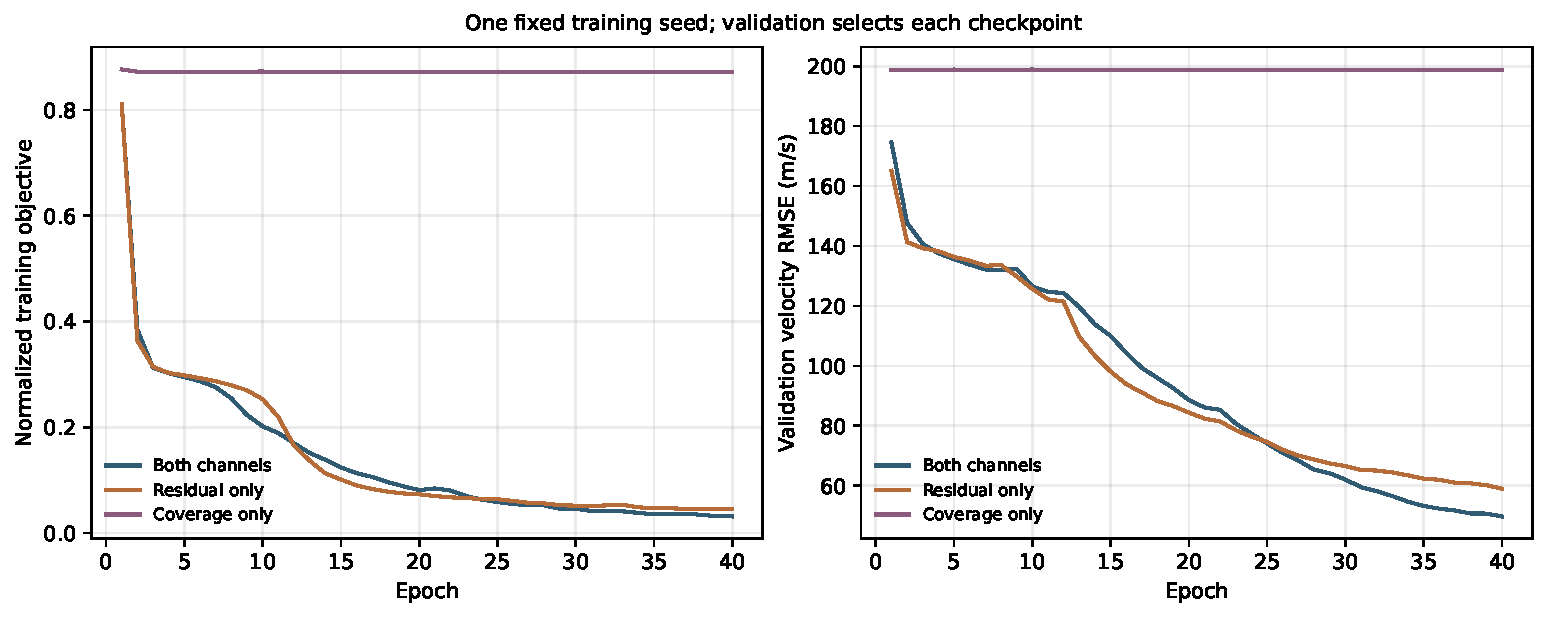
\includegraphics[width=0.98\textwidth]{figures/fig03-training-history.pdf}
\caption{Training objective and validation velocity error by epoch show the selected checkpoints for the full and channel-restricted networks.}
\label{fig:training}
\end{figure}

\begin{figure}[htbp]
\centering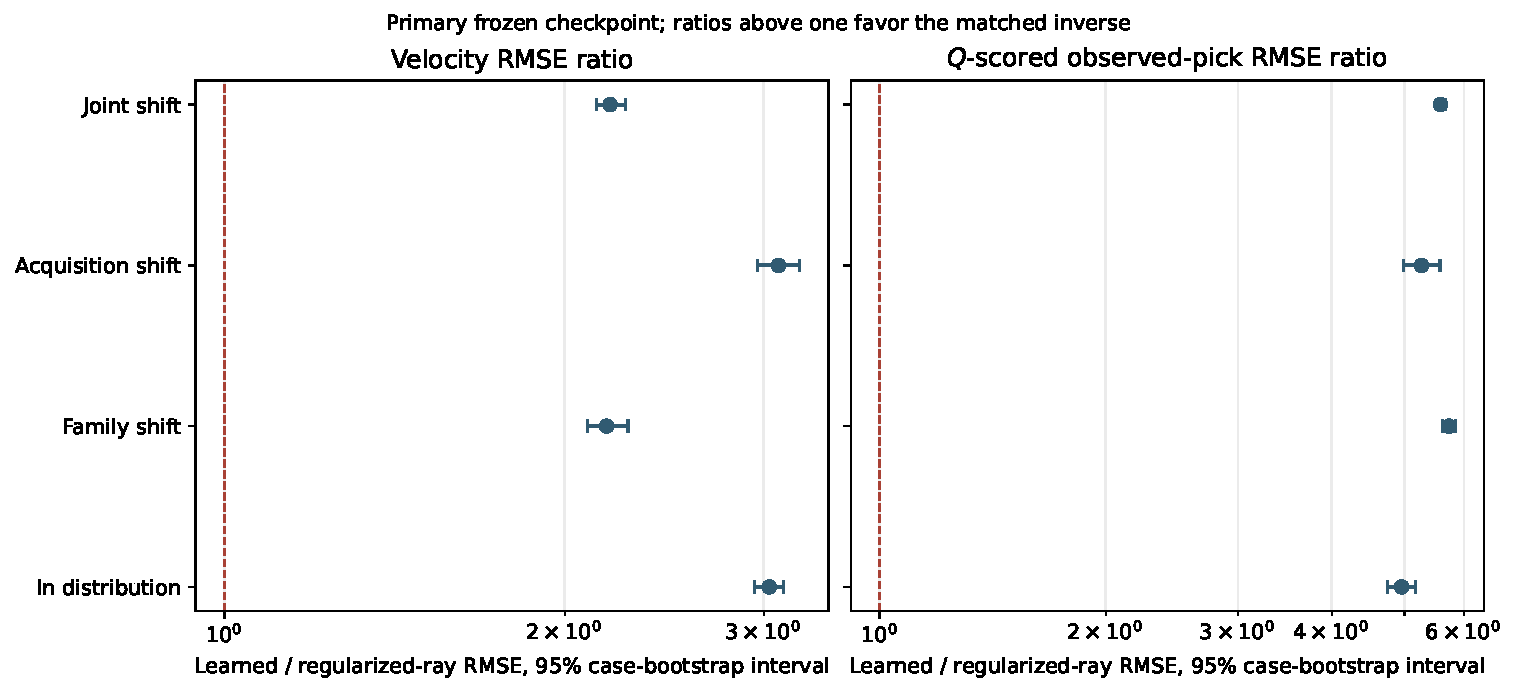
\includegraphics[width=0.98\textwidth]{figures/fig04-primary-heldout-ratios.pdf}
\caption{Held-out learned-to-reference error ratios and case-bootstrap intervals exceed unity for each cohort and both reported error domains.}
\label{fig:primary-ratios}
\end{figure}

\begin{figure}[htbp]
\centering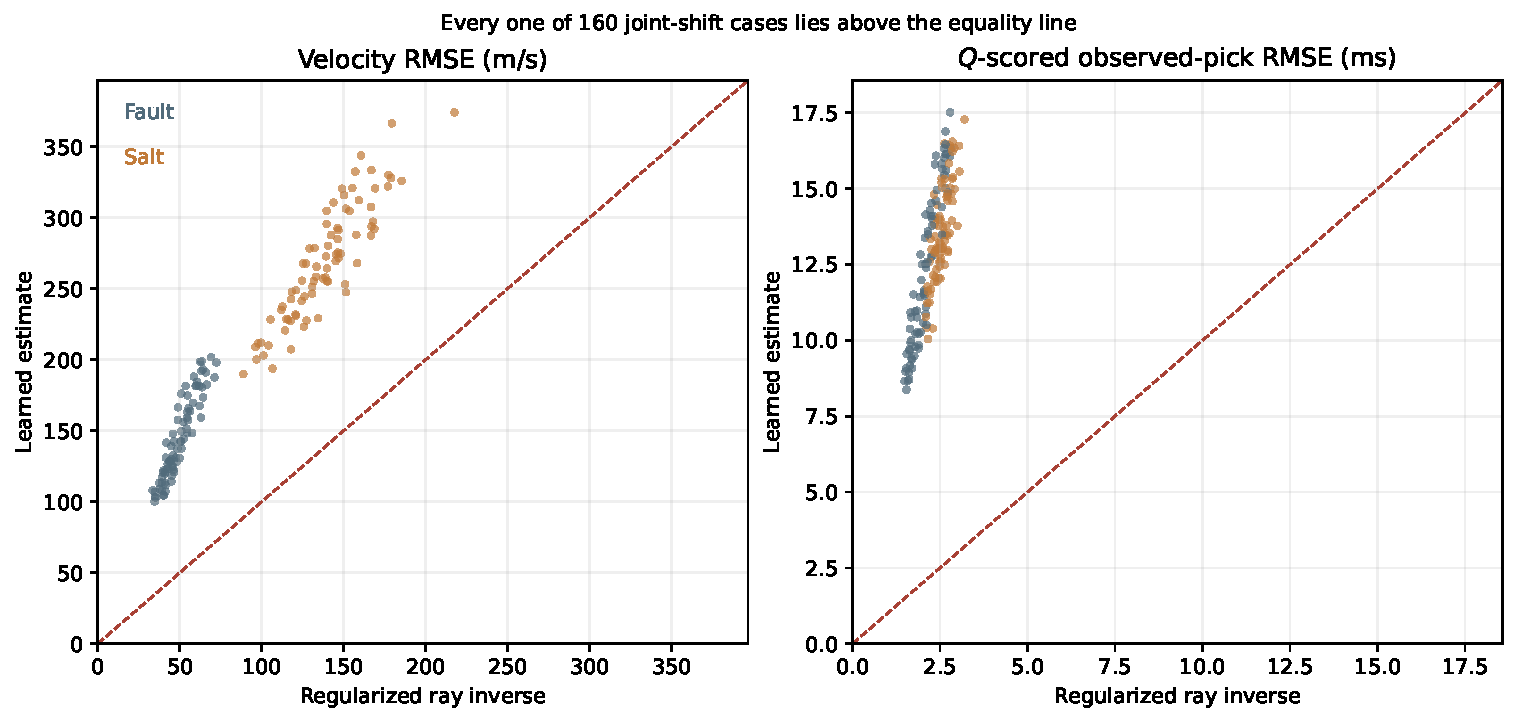
\includegraphics[width=0.98\textwidth]{figures/fig05-joint-shift-paired-errors.pdf}
\caption{Paired case errors on the joint family and acquisition shift compare velocity and $Q$-scored observed-pick travel-time RMSE against equality.}
\label{fig:paired-errors}
\end{figure}

\subsection{Training and diagnostic threshold}
\label{sec:training-results}
Training velocity RMSE on validation declines through the selected epoch, but its best value remains much larger than the reference's validation RMSE. The full model's validation errors show that ordinary interpolation within known families is also not solved by the selected checkpoint. The training objective includes a data term, yet training loss alone is not the evaluation criterion. Validation selects weights, the separately discretized $Q$ scorer evaluates observed-pick residuals, and test ratios determine the prespecified conclusion. Figure~\ref{fig:training} plots the saved histories for the primary model and the two channel ablations; it is generated directly from the frozen numerical outputs.

The threshold of 6.091015 ms is calculated as the empirical 95th percentile of the 160 validation learned-model errors under the bilinear scorer. All primary joint-shift cases exceed it. This does not mean each case has a 95\% probability of error or that a classifier calibrated to field data has failed. It means the observed synthetic residuals fall above a fixed validation quantile. Because validation cases are finite and synthetic, threshold uncertainty is not represented by a separate threshold interval. A future calibration study would require repeated validation cohorts, realistic pick uncertainty, and field-specific external validation.

\section{Ablation}
\label{sec:ablation}
\subsection{Channel tests on new test-cohort seeds}
\label{sec:ablation-results}
The exploratory ablation isolates the two input channels while holding the architecture, seed, optimizer, training cohort, validation cohort, epoch budget, velocity bounds, and classical regularization value fixed. The residual-only model masks coverage; the coverage-only model masks the residual. Both are trained from scratch. A full-channel result is supplied by the primary checkpoint and evaluated on the same new ablation test-cohort seed bases. The test manifests are disjoint from the primary test manifests, but the family templates and acquisition design remain known.

Every ablation remains worse than the reference in both metrics and all four cohorts. On the new joint-shift test cohort, the full model gives ratios 2.216 for velocity and 5.597 for time. Residual-only gives 2.327 and 5.757. Coverage-only gives 3.597 and 12.765. The coverage-only model therefore loses substantially more on this cohort, consistent with the fact that a map of ray density alone does not encode the sign or magnitude of travel-time residuals. Removing coverage also does not rescue the full method: residual-only ratios remain above one. These results are shown for all cohorts in Figure~\ref{fig:ablation} and Table~\ref{tab:ablation}.

Threshold flags are reported in the same table only as diagnostics. Each variant uses its own validation-derived 95th-percentile threshold, so flag counts should not be interpreted as direct calibrated comparisons between variants. The case-bootstrap intervals on new ablation test-cohort realizations estimate within-cohort case sampling variation. They do not capture retraining variability because only one training seed was used, and the full-channel model was not retrained for the follow-up. Ablation training and scoring took 30.452 seconds on the recorded CUDA device. Neither single-channel variant rescues the result on these test cohorts; this post-hoc, single-training-seed ablation does not identify the general cause of the primary failure.

\begin{figure}[htbp]
\centering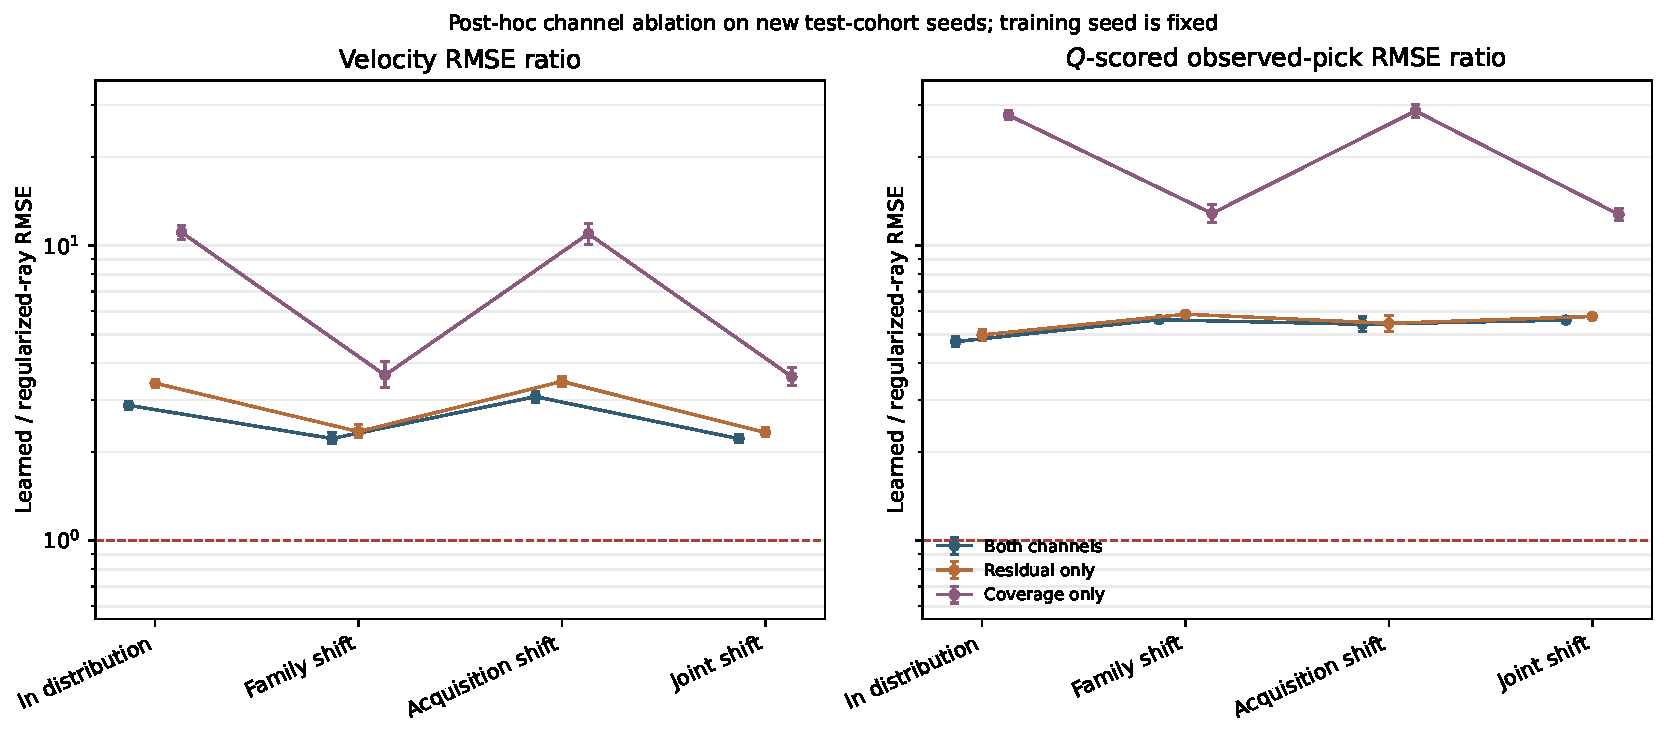
\includegraphics[width=0.98\textwidth]{figures/fig06-channel-ablation.pdf}
\caption{Channel-ablation ratios on new test-cohort seeds compare both inputs with residual-only and coverage-only variants over the four held-out cohort definitions; the training seed is fixed.}
\label{fig:ablation}
\end{figure}

\begin{figure}[htbp]
\centering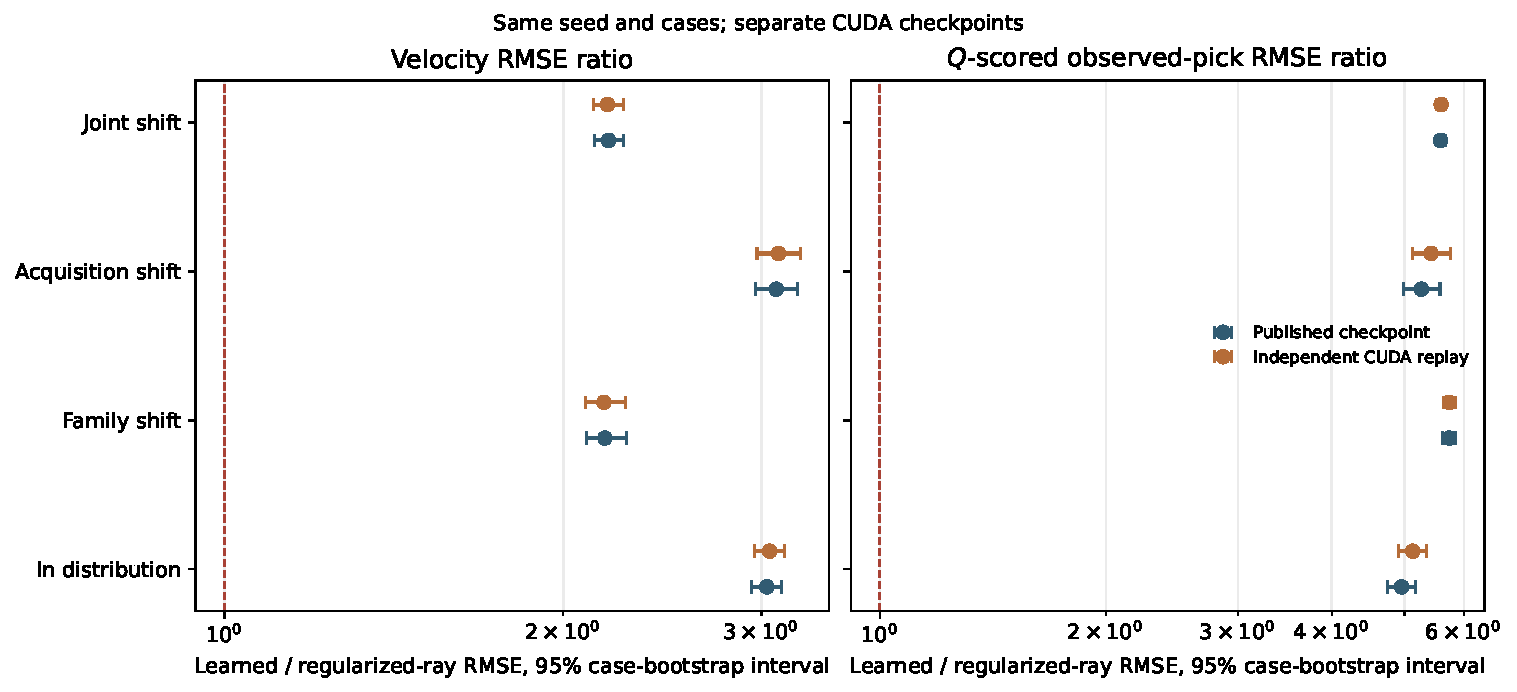
\includegraphics[width=0.98\textwidth]{figures/fig08-training-replay-sensitivity.pdf}
\caption{Case-bootstrap intervals compare two CUDA checkpoints trained with the same seed on identical cohorts; every ratio remains above unity.}
\label{fig:replay-sensitivity}
\end{figure}

\subsection{What the ablation does not establish}
\label{sec:ablation-limits}
The channel masks do not test alternative feature definitions, richer acquisition descriptors, nonlinear ray bending, deeper architectures, objective reweighting, a larger training distribution, transfer learning, uncertainty-aware losses, or a different solver family. They also do not separate architectural undercapacity from optimization difficulty or mismatch between cell-length training and bilinear scoring. The residual-only and coverage-only checkpoints are selected using the same validation velocity criterion, which is appropriate for the stated comparison but can select different epochs and different validation operating points.

Since the ablation was initiated after the primary negative result, it should be read as a follow-up diagnostic. New test-cohort seed bases reduce reuse of the original test records, but they do not erase the fact that choices about which channels to remove were informed by the observed outcome. The direction of its result is useful for planning a new preregistered study; its p-values, if any, would not convert it into a confirmatory experiment. No variant supports a method-superiority statement. The original failed comparison remains the primary result and is not replaced by the more favorable or less unfavorable metric of a selected subgroup.

\section{Discussion}
\label{sec:discussion}
The direct conclusion is that this geometry-normalized two-channel CNN does not improve on the matched regularized ray reference under the tested generator and frozen protocol. Both error ratios substantially exceed one on all held-out cohort definitions. The Q-scored residual is especially unfavorable. Because Q is separately discretized from A but also generates the synthetic observations, this check measures operator-discretization sensitivity rather than validation against a distinct physical data generator. At the same time, the test is small in spatial resolution, uses known families, and contains synthetic Gaussian pick errors. Its negative result should update confidence in this specific implementation, not serve as a universal ranking of machine learning and regularized inversion.

Several plausible mechanisms remain. The CNN may learn morphology that is correlated with training labels but not observable from the acquisition; the generator's salt and fault structures may be poorly represented by the layered, lens, and dipping training families; the 16 by 16 representation may make the residual feature too diffuse; and the bilinear scorer may expose discrepancies that are not optimized directly. The ablation suggests coverage alone is insufficient and that residual information alone is insufficient, but does not distinguish these explanations. A proper next experiment would vary one factor at a time under newly frozen splits and include multiple independent training seeds. It would also compare the same source/receiver data and noise realization across all solvers.

The reference itself is limited. A single first-difference quadratic penalty favours smooth models and its scalar strength is selected from only four values. Modified total variation, nonlinear ray tracing, eikonal solvers, ensemble methods, and probabilistic inversions can produce different tradeoffs [\cite{Jiang2016,Jiang2018,LiEKI2025,Zhao2022}]. The finite reference grid does not claim to be the best available baseline. The comparison is still informative because it asks whether the learned method beats a transparent baseline selected without test information, while a separately discretized numerical operator scores the outputs. Future comparisons should broaden the reference set while retaining matched observations, an explicitly specified scoring operator, and declared selection rules.

The display implication is important for scientific interfaces: model panels alone cannot show whether an estimate is constrained, whether its data prediction is consistent, or whether a learned prior has transferred. A useful workbench must connect the model, ray coverage, residuals, physical axes, and the baseline in the same view. Such a view makes assumptions inspectable, but visualization is not a substitute for reproducible computation or a validated uncertainty model. The current experiment supports a negative synthetic case study, not an operational recommendation for field surveys.

\section{Limitations}
\label{sec:limitations}
\subsection{Internal validity}
\label{sec:internal-validity}
The primary comparison uses one model-training seed and one checkpoint. Case bootstrap intervals do not include the variability induced by random initialization, mini-batch ordering, nondeterministic GPU kernels, or checkpoint selection. The baseline regularization value is selected by validation truth error, as is the model epoch; this gives both methods access to the same held-out-from-training but labeled validation cohort. This protocol is defensible for synthetic benchmarking, but it is not a field workflow where ground-truth velocity is unavailable. A future field-use selection criterion would need a data-only rule or independent calibration set.

The reference and scoring operators differ, but both are implemented from geometric paths and cell-centred slowness. The scoring operator is not a wave-equation simulator and does not account for finite-frequency sensitivity, attenuation, anisotropy, uncertainty correlation, source uncertainty, or pick-selection bias. The stated 1 ms noise is independent and homoscedastic. The test generator uses the same broad numerical assumptions for all methods. These choices isolate aspects of the learned inverse but simplify real seismic propagation. An independent CPU recomputation reproduced the per-case metrics within the specified cross-device tolerances. This supports numerical reproducibility of the stated setup, not its physical adequacy for a field survey.

\subsection{External and construct validity}
\label{sec:external-validity}
The grid is only 800 m by 800 m with 50 m cells and 128 prescribed straight rays per case. Training includes 800 models from three authored families and two acquisition layouts. The held-out families are fault and salt, both known by design. No raw field survey, independent geological model corpus, borehole constraint, or externally collected travel-time data enters training or scoring. Consequently, the results say nothing about how the checkpoint performs at a mine, basin, geothermal site, or earthquake network. Nor do they demonstrate that the synthetic families represent the distribution of real subsurface structures.

The endpoint is velocity RMSE and $Q$-scored misfit to noisy synthetic picks. These measures do not evaluate structural boundary accuracy, engineering decisions, uncertainty calibration, interpretive usefulness, or downstream migration/FWI performance. The residual threshold is not calibrated on field outcomes. The small grid and the output domain fixed by the generator may favour the convolutional architecture in some respects and disadvantage it in others. A model that satisfies the current ranges could still be geologically implausible, while a model with higher cellwise error might support a specific downstream task. No such task-specific evaluation was conducted.

\subsection{Statistical scope}
\label{sec:statistical-limits}
The 95\% intervals resample cases within each fixed cohort, treating cases as the exchangeable units for that generator condition. Within a cohort, family and acquisition assignments are deterministic functions of index and seed; cases are not a random sample from a known geological population. The intervals therefore summarize finite-case sensitivity under this sampling design and should not be read as population confidence intervals for the Earth. They also do not account for five correlated cohort definitions generated from related code or for post-hoc selection of the ablation. The main acceptance rule is descriptive and preregistered in the experiment specification, not a null-hypothesis significance test.

The intervals also condition on the selected regularization strength and neural checkpoint. They omit uncertainty introduced by choosing the best epoch on 160 validation models and selecting one of four baseline penalties. A nested repeated-seed analysis would resample training groups, repeat initialization and optimization, redo model selection inside each resample, and evaluate on a separate outer test set. That would estimate a different quantity and require its own preregistration and compute budget. The current case bootstrap must not be read as this more comprehensive analysis. The observed negative result is strong for the locked settings and finite cohorts, while variation under plausible retraining and model-selection choices remains unmeasured.

\section{Reproducibility and data availability}
\label{sec:reproducibility}
The source repository is \url{https://github.com/fsantibanezleal/CAOS_Geophysics}. The executable code and frozen data snapshot used for the reported numerical results are pinned to commit \texttt{41a5cad537b19aff35fc4f90535e8699ac4bf0e5}. The feature and generator implementation is in \url{data-pipeline/velocity_physics_refinement.py}; the ray and quadrature operators, families, and reference solver are in \url{data-pipeline/velocity_validation.py}. The ablation is implemented by \url{scripts/run_m12_physics_ablation.py}. The data subfolder contains frozen JSON numerical outputs and compact NumPy checkpoints. Their source and operator hashes are checked before any figure or table is created. A second independently trained checkpoint and its run metadata are included with SHA-256 values \texttt{b7d606a04fe66286490b62b5ddae89e9c4aca882c15afe56524f21f0e511beaf} and \texttt{d0b7905b80a184f01a761bb80430e7b6557fcc9dc00a88326f57c9bbdcf5975d}; cohort hashes match the primary run while checkpoint hashes differ. This commit is a reproducibility snapshot rather than an accepted product release, and no manuscript DOI is assigned.

Run \texttt{python}\ \texttt{build\_analysis.py} from the directory containing the analysis script. It regenerates eight vector PDF figures, PNG inspection copies, six result tables, and \url{generated/analysis.json}. Its paired percentile bootstrap uses 20,000 resamples and fixed PCG64 seeds. The included numerical files and checkpoints reproduce the reported summaries without access to the original external training folders. Regenerating the original training data from seed manifests and executing the model recomputation requires the repository's pinned Python environment and the commands in \url{docs/validation/bs1-learning-lesson-replay-2026-11-11.md} and \url{docs/validation/bs1-ablation-2026-11-11.md}. The primary CUDA training ran on an NVIDIA GeForce RTX 4070 Laptop GPU for 37.515 seconds; an independent CPU recomputation matched its per-case metrics within the recorded cross-device tolerances. The second CUDA execution took 22.542 seconds and produced the distinct checkpoint analysed above.

\section{Conclusions}
\label{sec:conclusions}
The tested residual network combines a path-length-normalized residual backprojection, normalized ray coverage, three convolutional residual blocks, and a bounded logit update around a reference velocity. It was trained and selected on 800 and 160 synthetic cases, then tested on four frozen cohort definitions. It did not improve on the validation-selected regularized ray reference. The joint family and acquisition cohort produced velocity and $Q$-scored travel-time RMSE ratios of 2.194 and 5.585 for the primary checkpoint and 2.190 and 5.595 for a second CUDA checkpoint trained with the same seed and tested on identical cases. All joint cases exceeded each run's validation-derived threshold. Single-channel ablations on new test-cohort seeds did not resolve the failure.

The experiment supports a narrow negative result for a known synthetic generator, fixed 16 by 16 model, straight-ray inversion, bilinear scoring operator, single training seed, and bounded protocol. It offers no field accuracy or geological-transfer evidence and no theoretical guarantee of benefit. Further work should test richer acquisition-aware parameterizations, nonlinear forward physics, repeated model-training seeds, more diverse and independently sourced structures, broader reference solvers, and field datasets with defensible uncertainty. Until such evidence exists, the learned output should be treated as an exploratory synthetic estimate rather than a validated field interpretation.

\begin{thebibliography}{99}
\bibitem{AkiLee1976} K. Aki and W. H. K. Lee, ``Determination of three-dimensional velocity anomalies under a seismic array using first P arrival times from local earthquakes, 1. A homogeneous initial model,'' \emph{Journal of Geophysical Research}, 81, 4381--4399, 1976. \href{https://doi.org/10.1029/JB081i023p04381}{doi:10.1029/JB081i023p04381}.
\bibitem{AkiChristofferson1977} K. Aki, A. Christofferson, and E. S. Husebye, ``Determination of the three-dimensional seismic structure of the lithosphere,'' \emph{Journal of Geophysical Research}, 82, 277--296, 1977. \href{https://doi.org/10.1029/JB082i002p00277}{doi:10.1029/JB082i002p00277}.
\bibitem{BackusGilbert1968} G. E. Backus and J. F. Gilbert, ``The resolving power of gross earth data,'' \emph{Geophysical Journal of the Royal Astronomical Society}, 16, 169--205, 1968. \href{https://doi.org/10.1111/j.1365-246X.1968.tb00216.x}{doi:10.1111/j.1365-246X.1968.tb00216.x}.
\bibitem{Vidale1988} J. E. Vidale, ``Finite-difference calculation of travel times,'' \emph{Bulletin of the Seismological Society of America}, 78, 2062--2076, 1988. \href{https://doi.org/10.1785/BSSA0780062062}{doi:10.1785/BSSA0780062062}.
\bibitem{Podvin1991} P. Podvin and I. Lecomte, ``Finite difference computation of traveltimes in very contrasted velocity models: a massively parallel approach and its associated tools,'' \emph{Geophysical Journal International}, 105, 271--284, 1991. \href{https://doi.org/10.1111/j.1365-246X.1991.tb03461.x}{doi:10.1111/j.1365-246X.1991.tb03461.x}.
\bibitem{MoHarris2002} L.-W. Mo and J. M. Harris, ``Finite-difference calculation of direct-arrival traveltimes using the eikonal equation,'' \emph{Geophysics}, 67, 1270--1274, 2002. \href{https://doi.org/10.1190/1.1500389}{doi:10.1190/1.1500389}.
\bibitem{Hole1992} J. A. Hole, ``Nonlinear high-resolution three-dimensional seismic travel time tomography,'' \emph{Journal of Geophysical Research}, 97, 6553--6562, 1992. \href{https://doi.org/10.1029/92JB00235}{doi:10.1029/92JB00235}.
\bibitem{Dahlen2004} F. A. Dahlen, ``Resolution limit of traveltime tomography,'' \emph{Geophysical Journal International}, 157, 315--331, 2004. \href{https://doi.org/10.1111/j.1365-246X.2004.02214.x}{doi:10.1111/j.1365-246X.2004.02214.x}.
\bibitem{Rawlinson2010} N. Rawlinson, S. Pozgay, and S. Fishwick, ``Seismic tomography: a window into deep Earth,'' \emph{Physics of the Earth and Planetary Interiors}, 178, 101--135, 2010. \href{https://doi.org/10.1016/j.pepi.2009.10.002}{doi:10.1016/j.pepi.2009.10.002}.
\bibitem{Menke2018} W. Menke, \emph{Geophysical Data Analysis: Discrete Inverse Theory}, 4th ed., Academic Press, 2018. ISBN 978-0-12-813555-6.
\bibitem{Aster2018} R. C. Aster, B. Borchers, and C. H. Thurber, \emph{Parameter Estimation and Inverse Problems}, 3rd ed., Elsevier, 2018. ISBN 978-0-12-804651-7.
\bibitem{Tikhonov1977} A. N. Tikhonov and V. Y. Arsenin, \emph{Solutions of Ill-Posed Problems}, Winston, 1977. ISBN 978-0-470-99124-4.
\bibitem{Hansen1992} P. C. Hansen, ``Analysis of discrete ill-posed problems by means of the L-curve,'' \emph{SIAM Review}, 34, 561--580, 1992. \href{https://doi.org/10.1137/1034115}{doi:10.1137/1034115}.
\bibitem{Constable1987} S. C. Constable, R. L. Parker, and C. G. Constable, ``Occam's inversion: a practical algorithm for generating smooth models from electromagnetic sounding data,'' \emph{Geophysics}, 52, 289--300, 1987. \href{https://doi.org/10.1190/1.1442303}{doi:10.1190/1.1442303}.
\bibitem{Jiang2016} W. Jiang and J. Zhang, ``First-arrival traveltime tomography with modified total-variation regularization,'' \emph{Geophysical Prospecting}, 65, 1138--1154, 2017. \href{https://doi.org/10.1111/1365-2478.12477}{doi:10.1111/1365-2478.12477}.
\bibitem{Jiang2018} W. Jiang and J. Zhang, ``3D first-arrival traveltime tomography with modified total variation regularization,'' \emph{Journal of Geophysics and Engineering}, 15, 207--223, 2018. \href{https://doi.org/10.1088/1742-2140/aa84d1}{doi:10.1088/1742-2140/aa84d1}.
\bibitem{TarantolaValette1982} A. Tarantola and B. Valette, ``Inverse problems = quest for information,'' \emph{Journal of Geophysics}, 50, 159--170, 1982. Stable URL: \url{https://journal.geophysicsjournal.com/JofG/article/view/28}.
\bibitem{ScalesSnieder1997} J. A. Scales and R. Snieder, ``To Bayes or not to Bayes?'' \emph{Geophysics}, 62, 1045--1046, 1997. \href{https://doi.org/10.1190/1.6241045.1}{doi:10.1190/1.6241045.1}.
\bibitem{MosegaardTarantola1995} K. Mosegaard and A. Tarantola, ``Monte Carlo sampling of solutions to inverse problems,'' \emph{Journal of Geophysical Research}, 100, 12431--12447, 1995. \href{https://doi.org/10.1029/94JB03097}{doi:10.1029/94JB03097}.
\bibitem{FanYing2023} Y. Fan and L. Ying, ``Solving traveltime tomography with deep learning,'' \emph{Communications in Mathematics and Statistics}, 11, 3--19, 2023. \href{https://doi.org/10.1007/s40304-022-00329-z}{doi:10.1007/s40304-022-00329-z}.
\bibitem{Muller2023} A. P. O. Muller et al., ``Deep-Tomography: iterative velocity model building with deep learning,'' \emph{Geophysical Journal International}, 232, 975--989, 2023. \href{https://doi.org/10.1093/gji/ggac374}{doi:10.1093/gji/ggac374}.
\bibitem{LiEKI2025} X. Li et al., ``Seismic traveltime tomography based on ensemble Kalman inversion,'' \emph{Geophysical Journal International}, 240, 290--302, 2025. \href{https://doi.org/10.1093/gji/ggae329}{doi:10.1093/gji/ggae329}.
\bibitem{Zeng2026} Y. Zeng, M. Bai, and Y. Chen, ``EKtomo: a physics-informed neural network approach for robust crosswell travel-time tomography,'' \emph{Geophysical Prospecting}, 74, e70184, 2026. \href{https://doi.org/10.1111/1365-2478.70184}{doi:10.1111/1365-2478.70184}.
\bibitem{YangDNR2026} S. Yang, H. Zhang, L. Gao, Z. Chen, J. Qian, and H. Yang, ``Seismic traveltime tomography with deep neural network reparameterization: the method and its application to Central Chile,'' \emph{Journal of Geophysical Research: Solid Earth}, 131, e2026JB034630, 2026. \href{https://doi.org/10.1029/2026JB034630}{doi:10.1029/2026JB034630}.
\bibitem{YangDNRData2026} S. Yang, ``Seismic traveltime tomography with deep neural network reparameterization'' [data set], Zenodo, 2026. \href{https://doi.org/10.5281/zenodo.20686320}{doi:10.5281/zenodo.20686320}.
\bibitem{ZhangAdjoint2026} Q. Zhang, X. Ma, Y. Nie, and H. Dong, ``Adjoint-state eikonal-equation-based traveltime tomography on unstructured triangular meshes,'' \emph{Journal of Applied Geophysics}, 253, 106395, 2026. \href{https://doi.org/10.1016/j.jappgeo.2026.106395}{doi:10.1016/j.jappgeo.2026.106395}.
\bibitem{LiHungLeung2026} W. Li, K. K. T. Hung, and S. Leung, ``A multilayer level-set method for eikonal-based traveltime tomography,'' \emph{Journal of Computational Physics}, 560, 114941, 2026. \href{https://doi.org/10.1016/j.jcp.2026.114941}{doi:10.1016/j.jcp.2026.114941}.
\bibitem{TangNTK2026} J. Tang, ``Neural tangent kernel adaptive weight physics-informed neural network for traveltime tomography,'' \emph{Journal of Geophysical Prospecting}, 2(3), 273--282, 2026. \href{https://doi.org/10.1016/j.jgp.2026.05.007}{doi:10.1016/j.jgp.2026.05.007}.
\bibitem{WangReciprocity2026} Y. Wang, H. Geng, C. Song, and C. Liu, ``Reciprocity-aware PINN-based seismic traveltime tomography and uncertainty quantification for models with irregular topography,'' \emph{Geophysical Journal International}, 244(3), ggag015, 2026. \href{https://doi.org/10.1093/gji/ggag015}{doi:10.1093/gji/ggag015}.
\bibitem{WangReciprocityCode2026} Y. Wang et al., ``RA-MC-PINNtomo: official notebook-based implementation of reciprocity-aware traveltime tomography,'' GitHub repository, 2026. \url{https://github.com/wangyf2322/RA-MC-PINNtomo}.
\bibitem{KurosawaMimir2026} I. Kurosawa, ``Total generalized variation regularization closes the gap between neural-field and classical methods in seismic travel-time tomography,'' arXiv:2605.09960, 2026. \url{https://arxiv.org/abs/2605.09960}.
\bibitem{KurosawaMimirCode2026} I. Kurosawa, ``MIMIR: neural-field travel-time tomography with TGV regularization,'' GitHub repository, 2026. \url{https://github.com/ISAO9/mimir}.
\bibitem{WangSpace2026} Y. Wang, Z. Jia, B. Jiang, and W. Lu, ``Space correlation constrained physics informed neural network for seismic tomography,'' \emph{Journal of Geophysical Research: Machine Learning and Computation}, 3, e2025JH000855, 2026. \href{https://doi.org/10.1029/2025JH000855}{doi:10.1029/2025JH000855}.
\bibitem{Deng2022} C. Deng et al., ``OpenFWI: large-scale multi-structural benchmark datasets for seismic full waveform inversion,'' in \emph{Advances in Neural Information Processing Systems}, 2022. \url{https://github.com/lanl/OpenFWI}.
\bibitem{Zhao2022} X. Zhao, A. Curtis, and X. Zhang, ``Bayesian seismic tomography using normalizing flows,'' \emph{Geophysical Journal International}, 228, 213--239, 2022. \href{https://doi.org/10.1093/gji/ggab298}{doi:10.1093/gji/ggab298}.
\bibitem{WangPickNet2019} J. Wang et al., ``Deep learning for picking seismic arrival times,'' \emph{Journal of Geophysical Research: Solid Earth}, 124, 6612--6624, 2019. \href{https://doi.org/10.1029/2019JB017536}{doi:10.1029/2019JB017536}.
\bibitem{ZhuBeroza2019} W. Zhu and G. C. Beroza, ``PhaseNet: a deep-neural-network-based seismic arrival-time picking method,'' \emph{Geophysical Journal International}, 216, 261--273, 2019. \href{https://doi.org/10.1093/gji/ggy423}{doi:10.1093/gji/ggy423}.
\bibitem{McCann2017} M. T. McCann, K. H. Jin, and M. Unser, ``A review of convolutional neural networks for inverse problems in imaging,'' \emph{IEEE Signal Processing Magazine}, 34, 85--95, 2017. \href{https://doi.org/10.1109/MSP.2017.2760358}{doi:10.1109/MSP.2017.2760358}.
\bibitem{AdlerOktem2018} J. Adler and O. \"Oktem, ``Learned primal-dual reconstruction,'' \emph{IEEE Transactions on Medical Imaging}, 37, 1322--1332, 2018. \href{https://doi.org/10.1109/TMI.2018.2798647}{doi:10.1109/TMI.2018.2798647}.
\bibitem{Ongie2020} G. Ongie et al., ``Deep learning techniques for inverse problems in imaging,'' \emph{IEEE Journal on Selected Areas in Information Theory}, 1, 39--56, 2020. \href{https://doi.org/10.1109/JSAIT.2020.2991563}{doi:10.1109/JSAIT.2020.2991563}.
\bibitem{Arridge2019} S. Arridge et al., ``Solving inverse problems using data-driven models,'' \emph{Acta Numerica}, 28, 1--174, 2019. \href{https://doi.org/10.1017/S0962492919000059}{doi:10.1017/S0962492919000059}.
\end{thebibliography}
\end{document}
